\documentclass{beamer}
\usetheme{Madrid}
\usecolortheme{whale}

\usepackage{listings}
\usepackage{graphicx}
\usepackage{booktabs}
\usepackage{amsmath}
\usepackage{bm}
\usepackage{threeparttable}
\usepackage{tabularx}
\usepackage{makecell}

\graphicspath{{../notebooks/figures/}}

\title{Bayesian Neural Networks on Two Moons}
\subtitle{Laplace Approximation vs. Variational Inference}
\author{Deep Learning Analysis}
\date{\today}

\begin{document}

\frame{\titlepage}

% ------------------------------------------------------------
\begin{frame}{Overview}
\begin{itemize}
    \item Two Moons binary classification benchmark
    \item Two BNN paradigms:
    \begin{itemize}
        \item \textbf{Laplace Approximation:} laplace-torch -- post-hoc Gaussian around MAP
        \item \textbf{Variational Inference:} bayesian-torch -- Flipout + BBB with ELBO / AvUC
    \end{itemize}
    \item Common infrastructure: shared helper modules, PyTorch MLP with 2 hidden layers (50 units), ReLU activations
    \item Evaluation: Brier Score, Expected Calibration Error (ECE), Expected vs Actual Uncertainty metrics, OOD robustness
\end{itemize}
\end{frame}

% ------------------------------------------------------------
\begin{frame}{Dataset: Two Moons}
\begin{columns}
\column{0.45\textwidth}
\begin{itemize}
    \item Synthetic 2D binary classification from \texttt{sklearn.datasets.make\_moons}
    \item \textbf{Config:} $n=10{,}000$ samples, noise=0.3, random seed 42
    \item Train/val/test split: 6000/1000/2000
    \item Features standardized via \texttt{StandardScaler}
    \item OOD: uniform grid $[-3,3]^2$ covering the full uncertainty map
\end{itemize}
\column{0.55\textwidth}
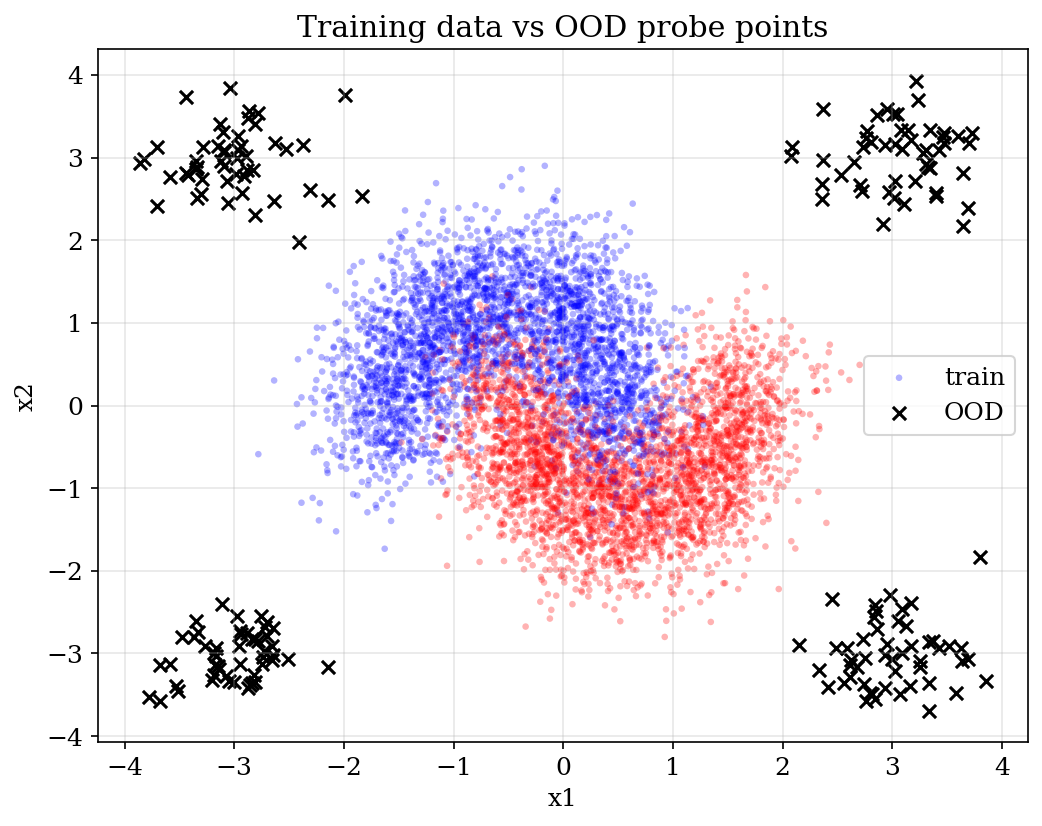
\includegraphics[width=\linewidth]{ood_points.png}
\end{columns}
\end{frame}

% ------------------------------------------------------------
\begin{frame}{Background: Laplace Approximation}
\begin{block}{Post-hoc Gaussian Posterior}
Given a MAP estimate $\bm{\theta}_{\text{MAP}}$, the Laplace approximation constructs
\[
p(\bm{\theta} \mid \mathcal{D}) \;\approx\; \mathcal{N}\!\bigl(\bm{\theta}_{\text{MAP}},\; \mathbf{H}^{-1}\bigr),
\qquad
\mathbf{H} = \nabla^2_{\bm{\theta}} \bigl[-\log p(\mathcal{D}\mid\bm{\theta})\bigr]\big|_{\bm{\theta}_{\text{MAP}}}
\]
\end{block}
\begin{block}{Hessian Approximations}
\begin{itemize}
    \item \textbf{Diag:} diagonal of GGN -- fast, $O(d)$ storage
    \item \textbf{Kron:} Kronecker-factor eigendecomposition of GGN -- moderate, $O(d^{3/2})$
    \item \textbf{Full:} full GGN matrix -- expensive, $O(d^2)$ storage
\end{itemize}
Tuning via gridsearch vs.\ marglik.
\end{block}
\end{frame}

% ------------------------------------------------------------
\begin{frame}{Background: ELBO Objective}
The Evidence Lower Bound (ELBO) for variational inference:
\[
\mathcal{L}_{\text{ELBO}}(\bm{\phi}) = \underbrace{\mathbb{E}_{q_{\bm{\phi}}(\bm{\theta})}\bigl[\log p(\mathcal{D}\mid\bm{\theta})\bigr]}_{\text{Expected log-likelihood}} \;-\; \underbrace{D_{\text{KL}}\bigl(q_{\bm{\phi}}(\bm{\theta}) \;\|\; p(\bm{\theta})\bigr)}_{\text{KL divergence to prior}}
\]
where:
\begin{itemize}
    \item $q_{\bm{\phi}}(\bm{\theta})$ -- variational posterior (Gaussian with learned mean/variance)
    \item $p(\bm{\theta})$ -- isotropic Gaussian prior
    \item Reparameterization trick enables gradient-based optimisation
    \item Flipout: decorrelates gradients within each mini-batch for lower-variance updates
    \item BBB: local reparameterization for computational efficiency
\end{itemize}
\end{frame}

% ------------------------------------------------------------
\begin{frame}{Background: AvUC Loss}
Accuracy vs.\ Uncertainty (AvUC) augments the ELBO to penalise mis-calibrated uncertainty:
\[
\mathcal{L}_{\text{AvUC}} = \mathcal{L}_{\text{ELBO}} + \lambda \cdot \mathcal{L}_{\text{U}}
\]
where the uncertainty regularisation term $\mathcal{L}_{\text{U}}$ is:
\[
\mathcal{L}_{\text{U}} = \sum_{b=1}^{B} \Bigl|\, \text{Acc}(b) - \text{Unc}(b) \,\Bigr|
\]
with:
\begin{itemize}
    \item $B$ bins partitioning $(0,1)$ by confidence level
    \item $\text{Acc}(b)$ -- accuracy of samples in bin $b$
    \item $\text{Unc}(b)$ -- average uncertainty ($1-\text{confidence}$) of samples in bin $b$
    \item $\lambda$ balances likelihood fit vs.\ calibration
\end{itemize}
\textbf{MOPED initialisation:} $\sigma_i^{\text{prior}} = \delta \cdot |\theta_{\text{MAP}}^{(i)}|$ with $\delta=0.5$ -- per-weight data-driven prior scale.
\end{frame}

% ------------------------------------------------------------
\begin{frame}{Metrics: Brier Score and ECE}
\textbf{Brier Score} -- mean squared error between predicted probabilities and one-hot labels:
\[
\text{BS} = \frac{1}{N}\sum_{n=1}^{N}\sum_{c=1}^{C}\bigl(\hat{p}_{nc} - \mathbf{1}[y_n=c]\bigr)^2
\]
where $\hat{p}_{nc}$ is the predicted probability for class $c$ on sample $n$, and $\mathbf{1}[y_n=c]$ is the indicator.
Lower is better.

\vspace{0.3cm}
\textbf{Expected Calibration Error (ECE)} -- average absolute gap between accuracy and confidence across $B$ bins:
\[
\text{ECE} = \sum_{b=1}^{B} \frac{|b|}{N}\; \bigl|\,\text{acc}(b) - \text{conf}(b)\,\bigr|
\]
where $\text{acc}(b) = \frac{1}{|b|}\sum_{n\in b}\mathbf{1}[\hat{y}_n=y_n]$ and $\text{conf}(b) = \frac{1}{|b|}\sum_{n\in b}\hat{p}_{n\hat{y}_n}$.
\end{frame}

% ------------------------------------------------------------
\begin{frame}{Metrics: Expected vs Actual Uncertainty}
Let $\text{gap}_b = |\text{acc}(b) - \text{unc}(b)|$ for each bin $b$, where $\text{unc}(b) = 1 - \text{conf}(b)$, and $B = 15$ bins (evenly spaced by confidence, per notebooks).

\vspace{-0.2cm}
\[
\text{U-MAE} = \frac{1}{B}\sum_{b=1}^{B} \text{gap}_b, \qquad
\text{U-MSE} = \frac{1}{B}\sum_{b=1}^{B} \text{gap}_b^2
\]

Mean absolute / squared deviation between expected and actual uncertainty.

\vspace{0.1cm}
\[
\text{U-Corr} = \text{Corr}\bigl(\{\text{acc}(b)\},\;\{\text{unc}(b)\}\bigr), \qquad
\text{MaxGap} = \max_{b=1,\dots,B} \text{gap}_b
\]

Correlation between accuracy and uncertainty (higher = better); worst-case calibration gap.
\end{frame}

% ------------------------------------------------------------
\begin{frame}{Laplace Configurations}
All trained on MAP (SGD, lr=0.01, 100 epochs), then Hessian is fit on the training set.
\begin{table}
\centering
\small
\begin{tabular}{lll}
\toprule
\textbf{Variant} & \textbf{Hessian} & \textbf{Scope} \\
\midrule
Diag / all / GS & Diagonal & All weights \\
Full / all / GS & Full GGN & All weights \\
Kron / all / GS & Kronecker & All weights \\
Full / LL / GS & Full GGN & Last layer only \\
Kron / LL / GS & Kronecker & Last layer only \\
\bottomrule
\end{tabular}
\end{table}
All five GS variants produce nearly identical metrics (identical Hessian fit).
\end{frame}

% ------------------------------------------------------------
\begin{frame}{Laplace Calibration Metrics (Gridsearch)}
\begin{threeparttable}
\centering
\small
\begin{tabular}{lccccc}
\toprule
\textbf{Variant} & \textbf{BS$\downarrow$} & \textbf{ECE$\downarrow$} & \textbf{U-MAE$\downarrow$} & \textbf{U-MSE$\downarrow$} & \textbf{U-Corr$\uparrow$} \\
\midrule
Diag / all / GS & 0.0564 & 0.0101 & 0.0101 & 0.0008 & 0.959 \\
Full / all / GS & 0.0564 & 0.0101 & 0.0101 & 0.0008 & 0.959 \\
Kron / all / GS & 0.0564 & 0.0101 & 0.0101 & 0.0008 & 0.959 \\
Full / LL / GS & 0.0564 & 0.0101 & 0.0101 & 0.0008 & 0.959 \\
Kron / LL / GS & 0.0564 & 0.0101 & 0.0101 & 0.0008 & 0.959 \\
\bottomrule
\end{tabular}
\begin{tablenotes}
\small
\item[BS] Brier Score (lower is better); \;[ECE] Expected Calibration Error (lower is better);
\item[U-MAE / MSE] Mean absolute / squared uncertainty gap; \;[U-Corr] Correlation (higher is better).
\end{tablenotes}
\end{threeparttable}
\end{frame}

% ------------------------------------------------------------
\begin{frame}{Laplace Computational Metrics (Gridsearch)}
\begin{threeparttable}
\centering
\small
\begin{tabular}{lcccc}
\toprule
\textbf{Variant} & \textbf{MaxGap$\downarrow$} & \textbf{Fit (s)} & \textbf{Tune (s)} & \textbf{Inf (s)} \\
\midrule
Diag / all / GS & 0.197 & 0.23 & 4.01 & 0.021 \\
Full / all / GS & 0.197 & 1262.97 & 11.42 & 0.034 \\
Kron / all / GS & 0.197 & 0.54 & 5.29 & 0.022 \\
Full / LL / GS & 0.197 & 7.12 & 1.52 & 0.001 \\
Kron / LL / GS & 0.197 & 0.43 & 1.85 & 0.001 \\
\bottomrule
\end{tabular}
\begin{tablenotes}
\small
\item[MaxGap] Worst-case bin calibration gap; \;[Fit/Tune/Inf] Train, hyperparameter, inference time.
\end{tablenotes}
\end{threeparttable}
\end{frame}

% ------------------------------------------------------------
\begin{frame}{Diag / all / GS}
\begin{columns}
\column{0.5\textwidth}
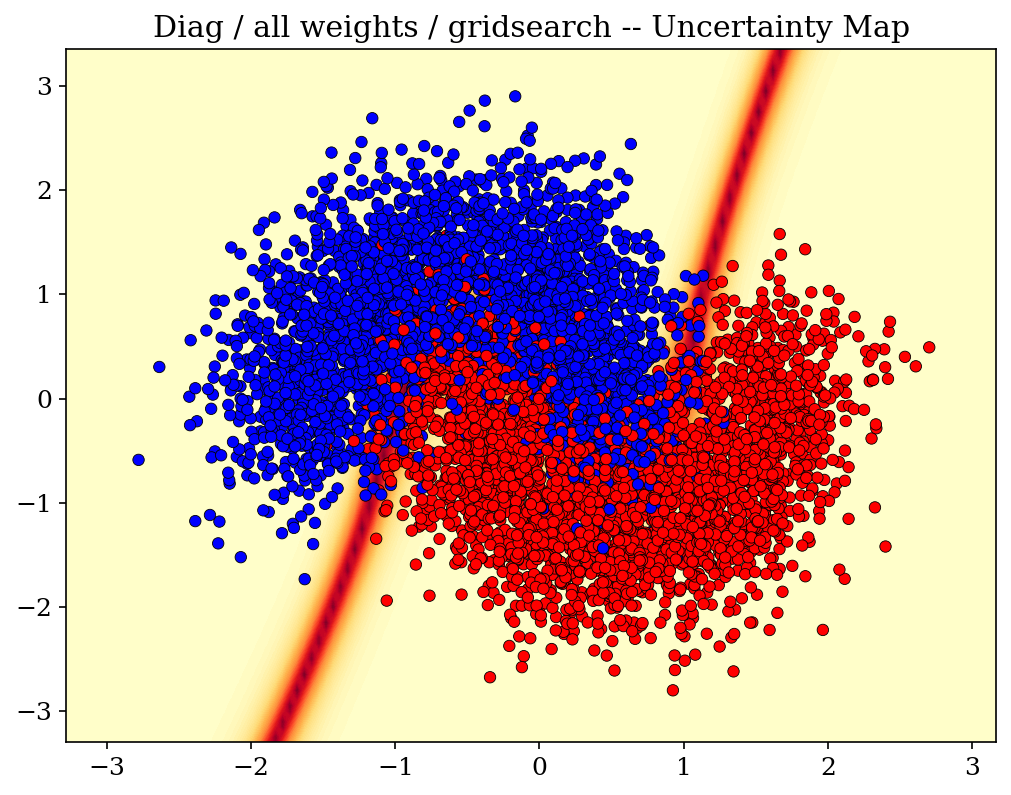
\includegraphics[width=\linewidth]{gridsearch_diag_all_weights_uncertainty.png}
\centerline{\tiny Uncertainty map ($1 - \max_c \hat{p}_c$)}
\column{0.5\textwidth}
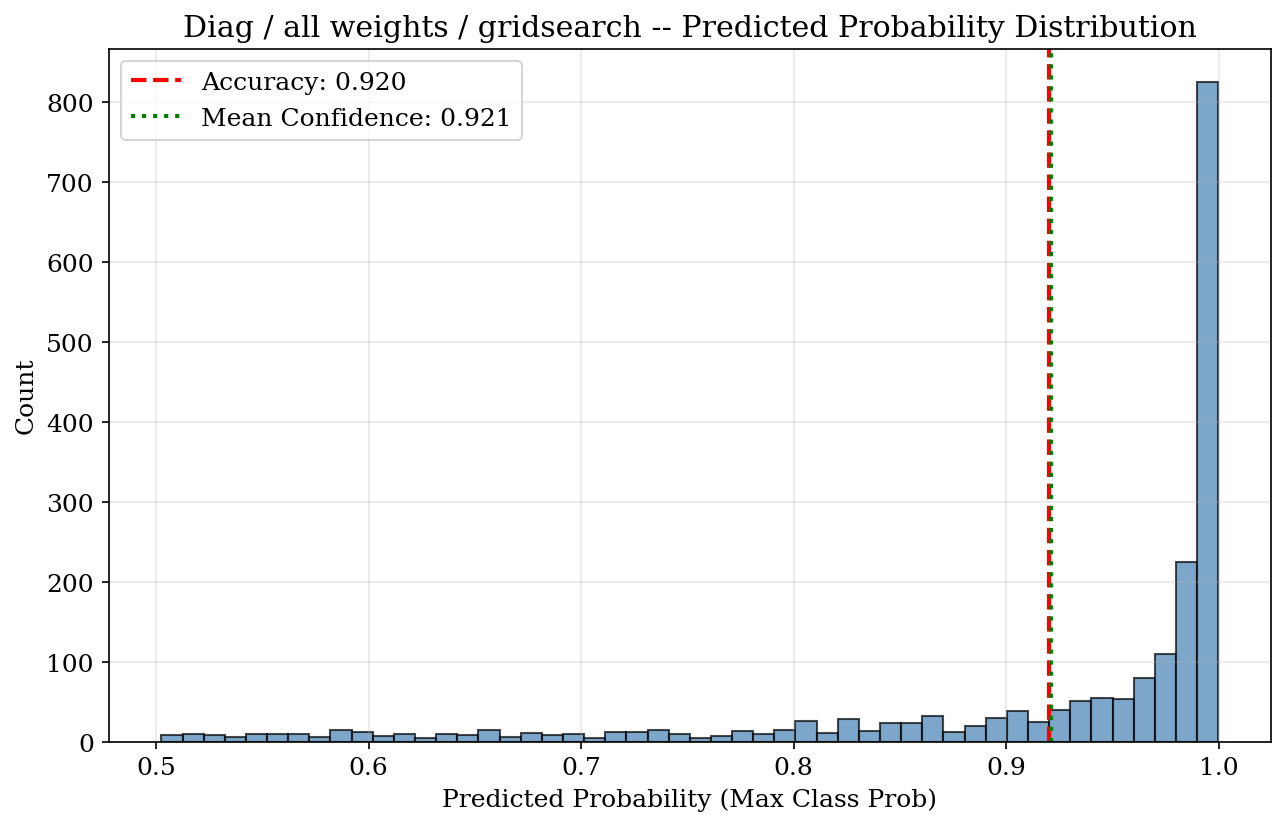
\includegraphics[width=\linewidth]{gridsearch_diag_all_weights_histogram.png}
\centerline{\tiny Prediction confidence histogram}
\end{columns}
\end{frame}

% ------------------------------------------------------------
\begin{frame}{Full / all / GS}
\begin{columns}
\column{0.5\textwidth}
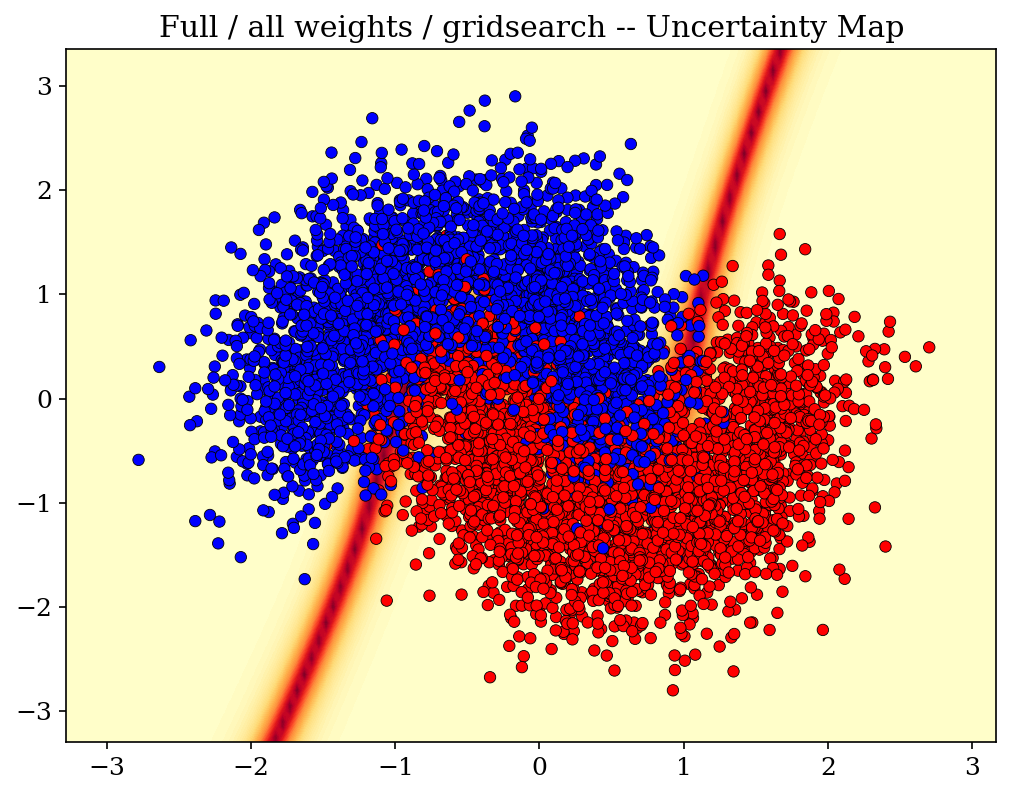
\includegraphics[width=\linewidth]{gridsearch_full_all_weights_uncertainty.png}
\centerline{\tiny Uncertainty map ($1 - \max_c \hat{p}_c$)}
\column{0.5\textwidth}
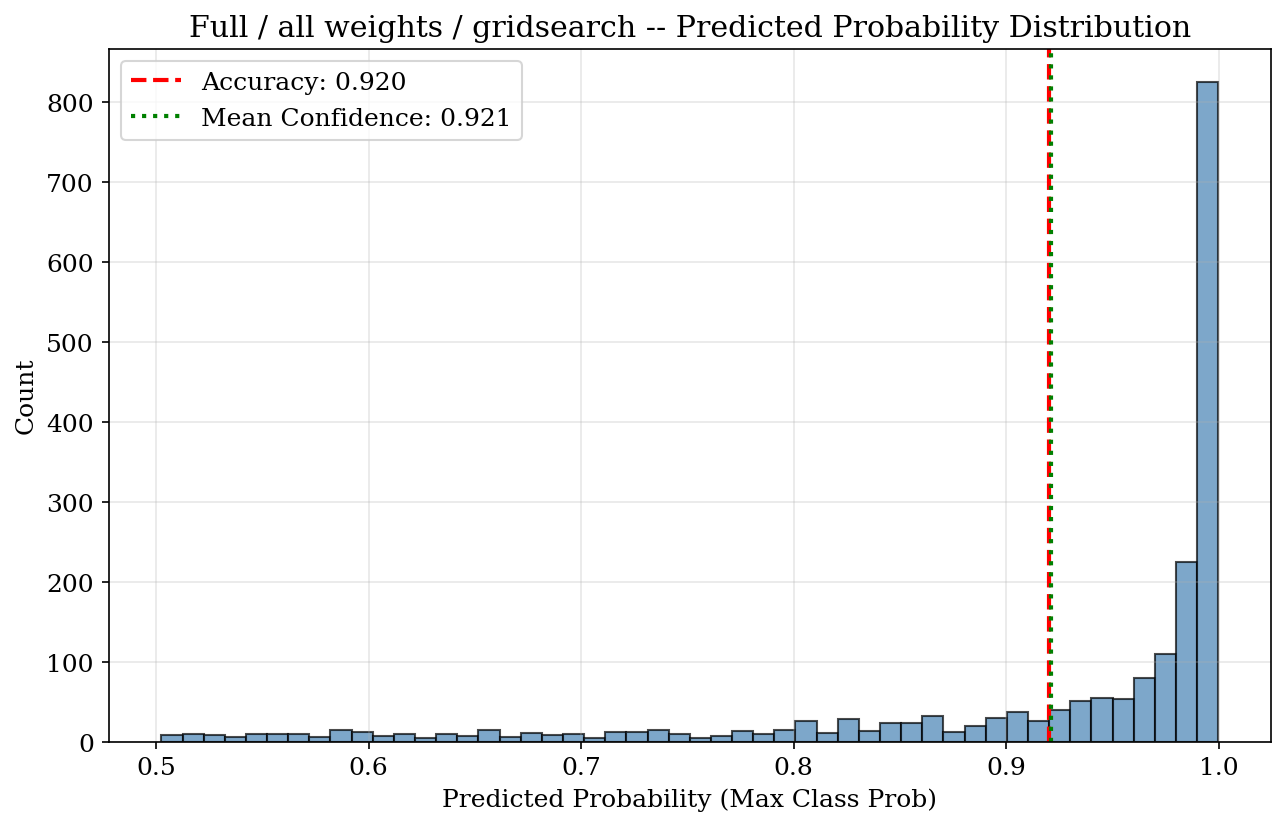
\includegraphics[width=\linewidth]{gridsearch_full_all_weights_histogram.png}
\centerline{\tiny Prediction confidence histogram}
\end{columns}
\end{frame}

% ------------------------------------------------------------
\begin{frame}{Kron / all / GS}
\begin{columns}
\column{0.5\textwidth}
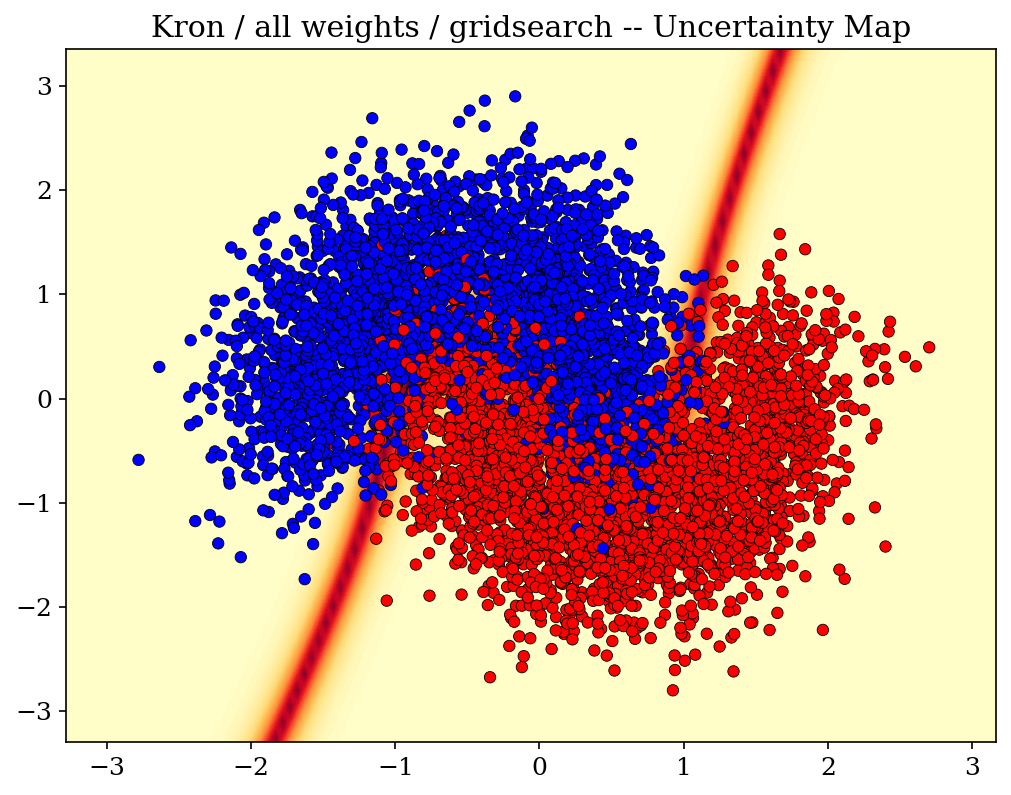
\includegraphics[width=\linewidth]{gridsearch_kron_all_weights_uncertainty.png}
\centerline{\tiny Uncertainty map ($1 - \max_c \hat{p}_c$)}
\column{0.5\textwidth}
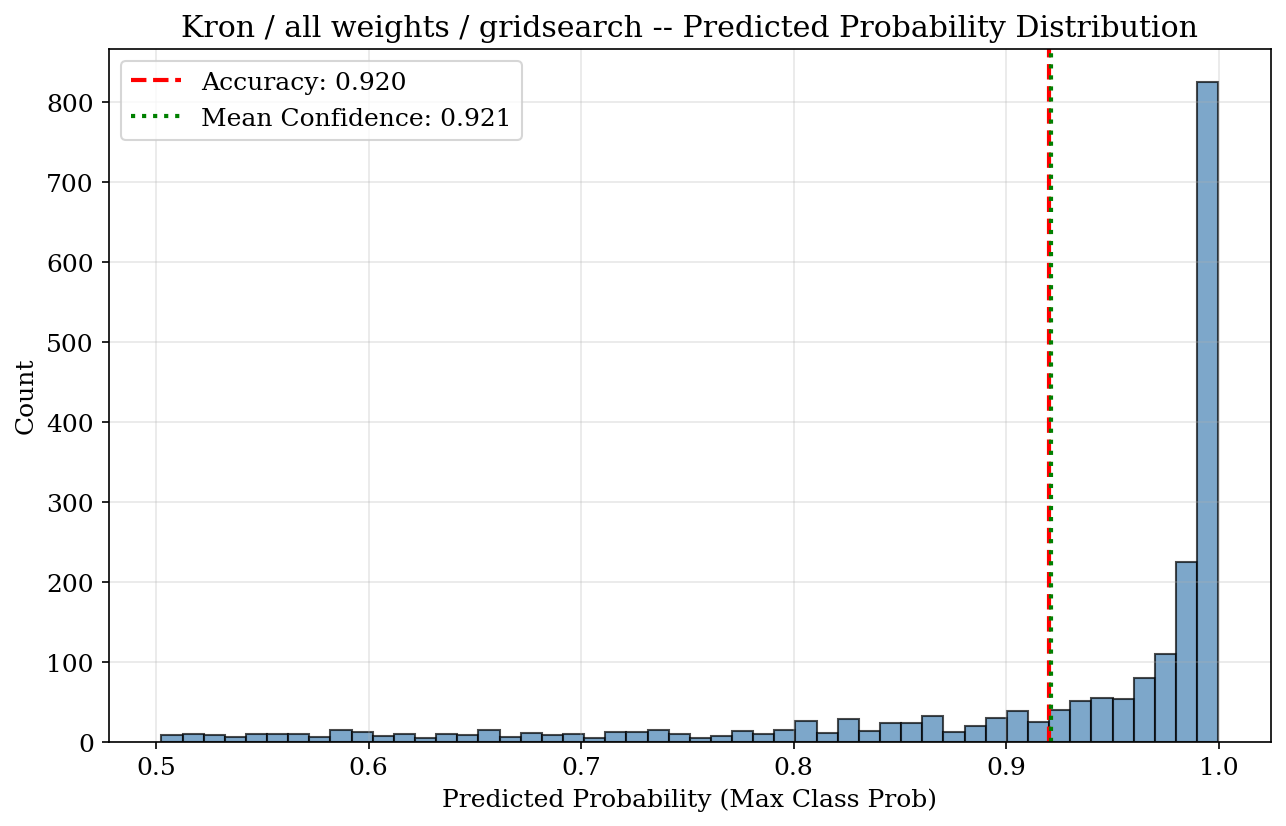
\includegraphics[width=\linewidth]{gridsearch_kron_all_weights_histogram.png}
\centerline{\tiny Prediction confidence histogram}
\end{columns}
\end{frame}

% ------------------------------------------------------------
\begin{frame}{Full / LL / GS}
\begin{columns}
\column{0.5\textwidth}
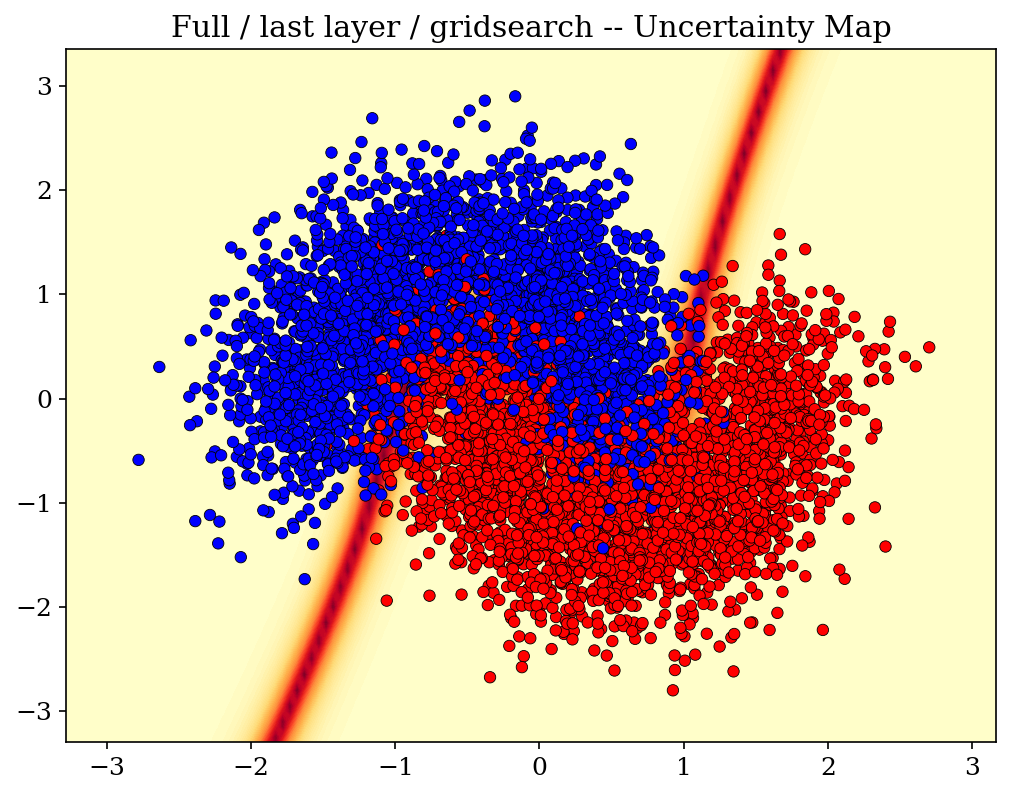
\includegraphics[width=\linewidth]{gridsearch_full_last_layer_uncertainty.png}
\centerline{\tiny Uncertainty map ($1 - \max_c \hat{p}_c$)}
\column{0.5\textwidth}
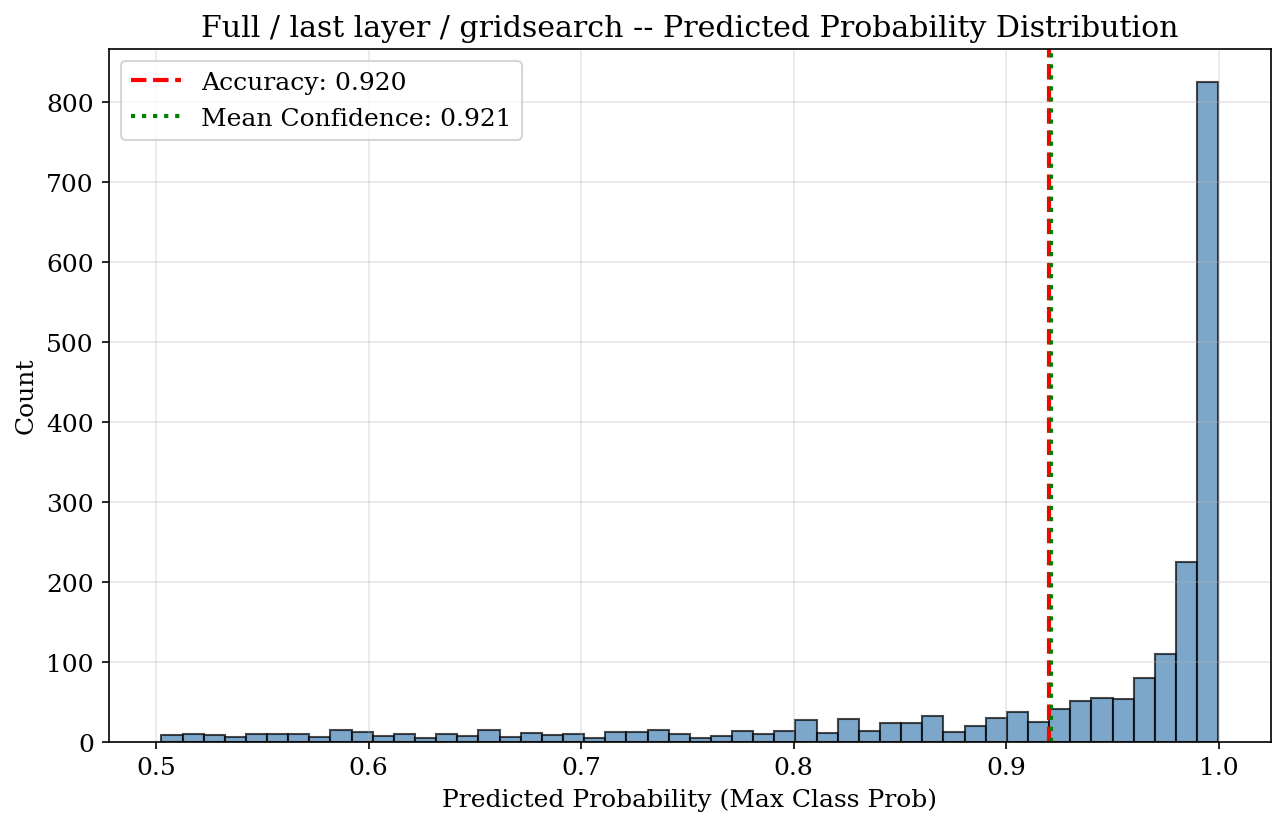
\includegraphics[width=\linewidth]{gridsearch_full_last_layer_histogram.png}
\centerline{\tiny Prediction confidence histogram}
\end{columns}
\end{frame}

% ------------------------------------------------------------
\begin{frame}{Kron / LL / GS}
\begin{columns}
\column{0.5\textwidth}
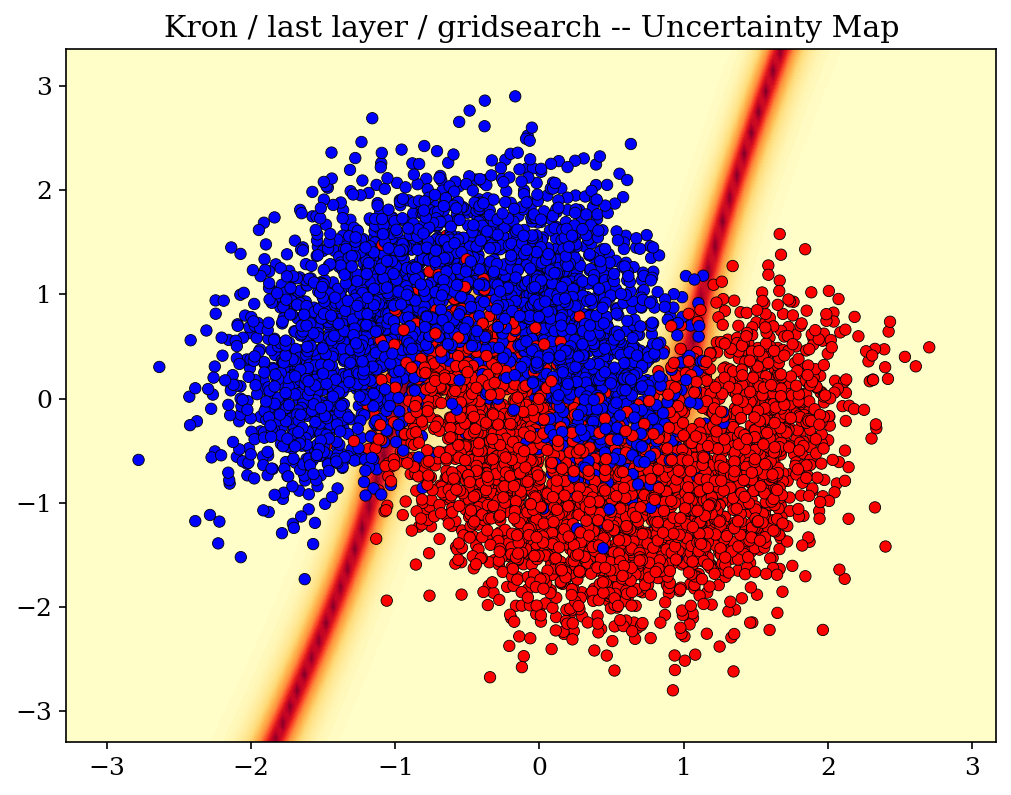
\includegraphics[width=\linewidth]{gridsearch_kron_last_layer_uncertainty.png}
\centerline{\tiny Uncertainty map ($1 - \max_c \hat{p}_c$)}
\column{0.5\textwidth}
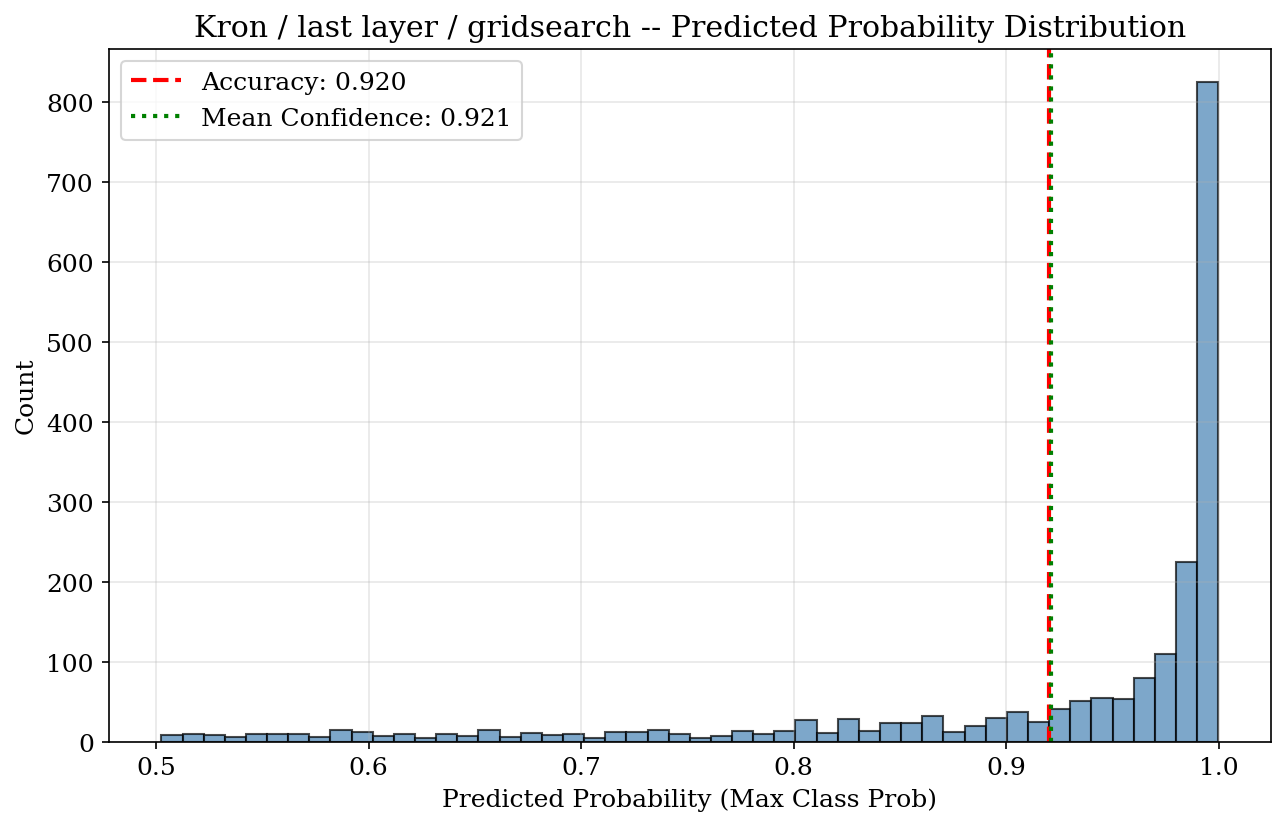
\includegraphics[width=\linewidth]{gridsearch_kron_last_layer_histogram.png}
\centerline{\tiny Prediction confidence histogram}
\end{columns}
\end{frame}

% ------------------------------------------------------------
\begin{frame}{Diag / all / ML}
\begin{columns}
\column{0.5\textwidth}
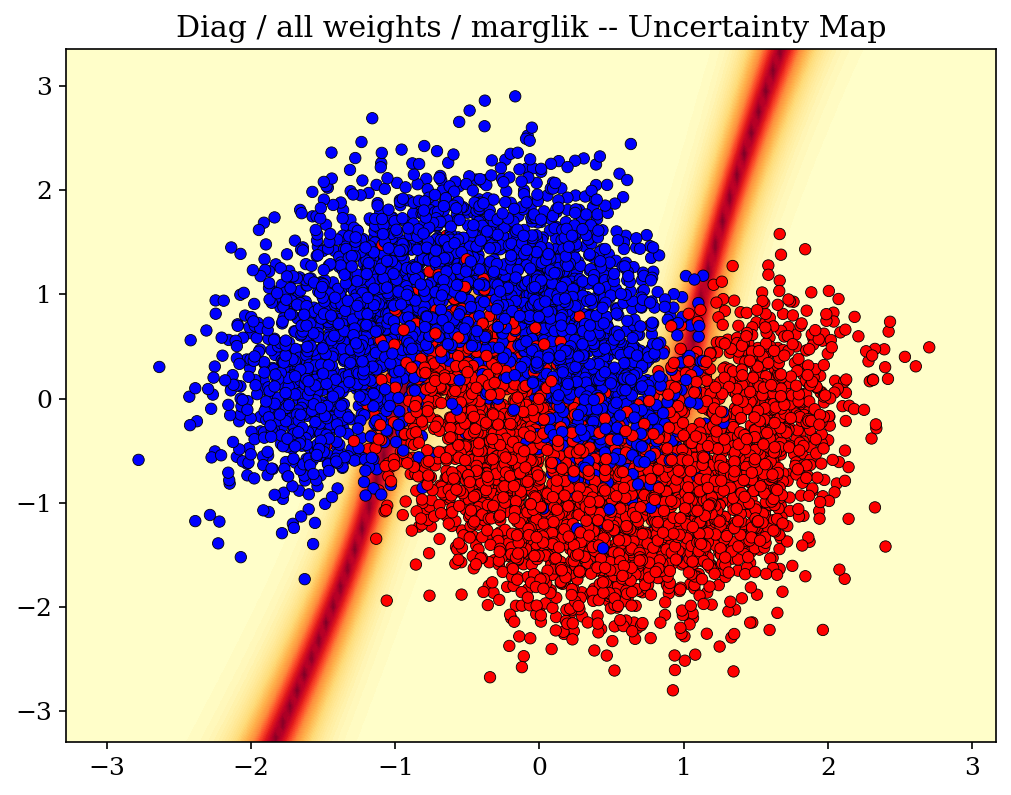
\includegraphics[width=\linewidth]{marglik_diag_all_weights_uncertainty.png}
\centerline{\tiny Uncertainty map ($1 - \max_c \hat{p}_c$)}
\column{0.5\textwidth}
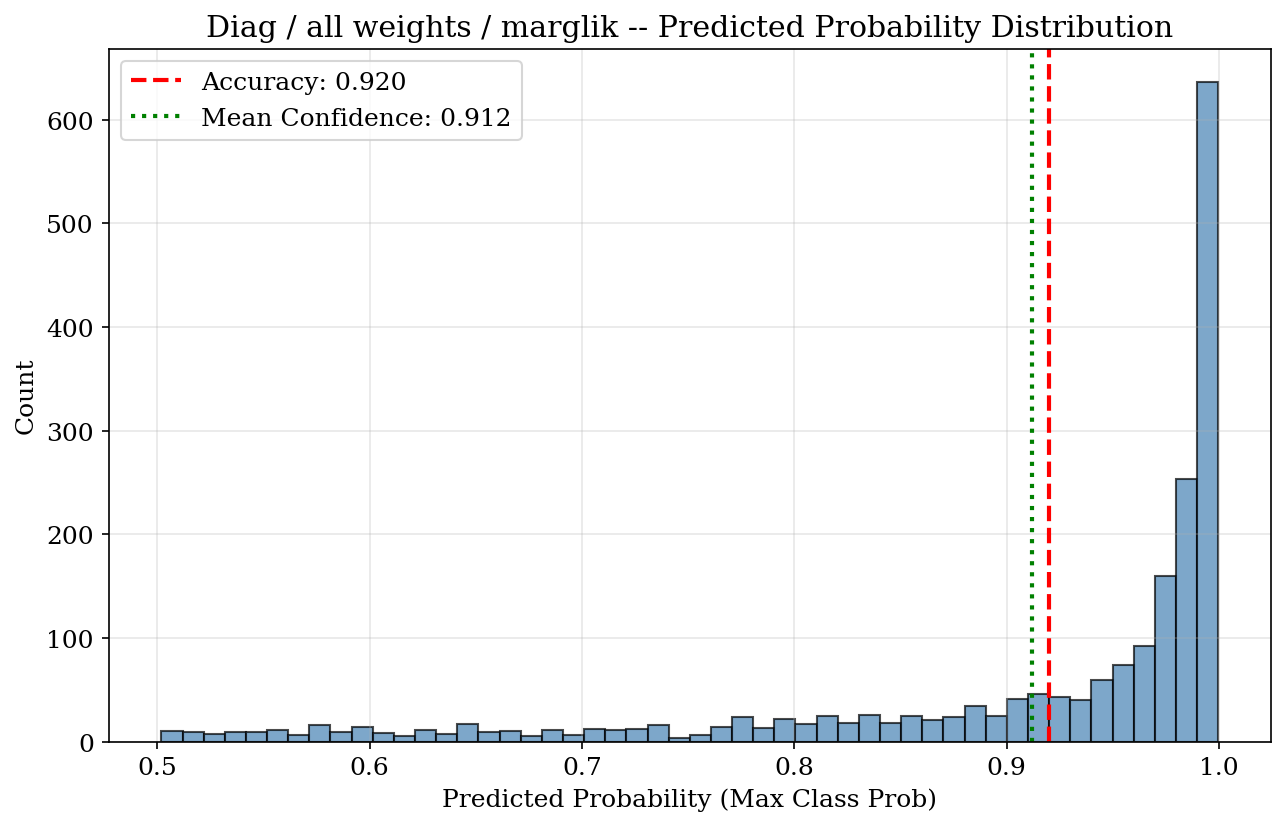
\includegraphics[width=\linewidth]{marglik_diag_all_weights_histogram.png}
\centerline{\tiny Prediction confidence histogram}
\end{columns}
\end{frame}

% ------------------------------------------------------------
\begin{frame}{Full / all / ML}
\begin{columns}
\column{0.5\textwidth}
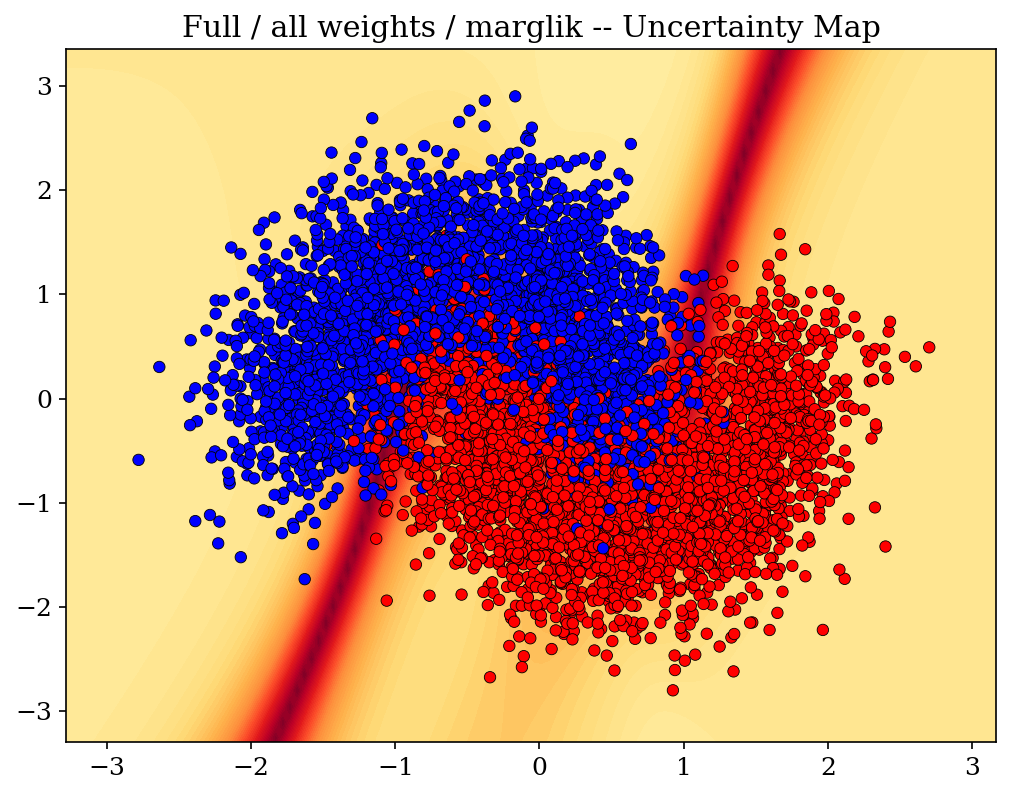
\includegraphics[width=\linewidth]{marglik_full_all_weights_uncertainty.png}
\centerline{\tiny Uncertainty map ($1 - \max_c \hat{p}_c$)}
\column{0.5\textwidth}
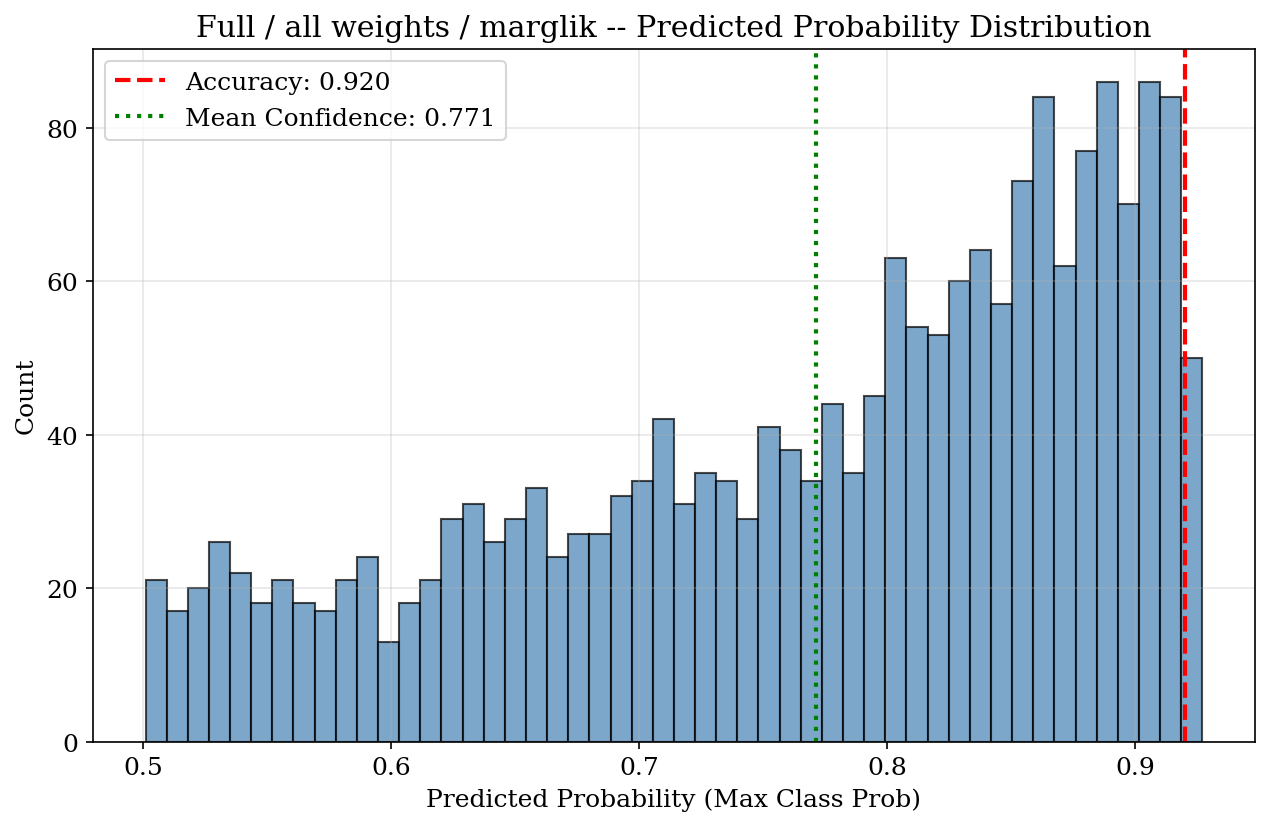
\includegraphics[width=\linewidth]{marglik_full_all_weights_histogram.png}
\centerline{\tiny Prediction confidence histogram}
\end{columns}
\end{frame}

% ------------------------------------------------------------
\begin{frame}{Kron / all / ML}
\begin{columns}
\column{0.5\textwidth}
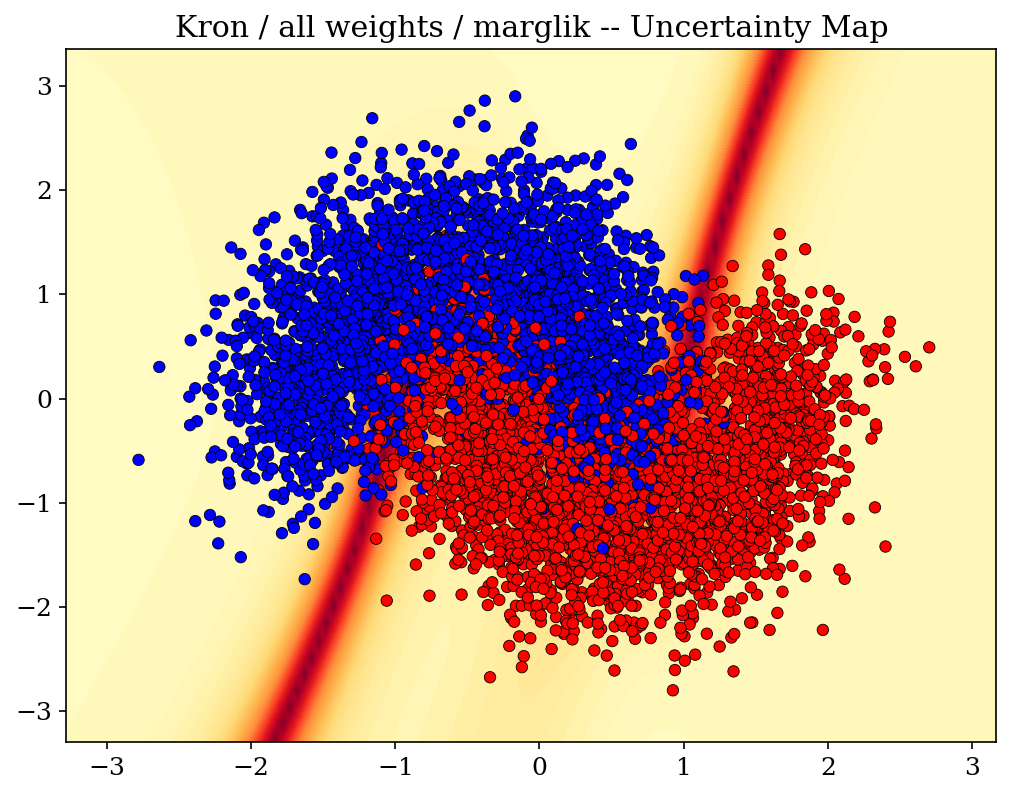
\includegraphics[width=\linewidth]{marglik_kron_all_weights_uncertainty.png}
\centerline{\tiny Uncertainty map ($1 - \max_c \hat{p}_c$)}
\column{0.5\textwidth}
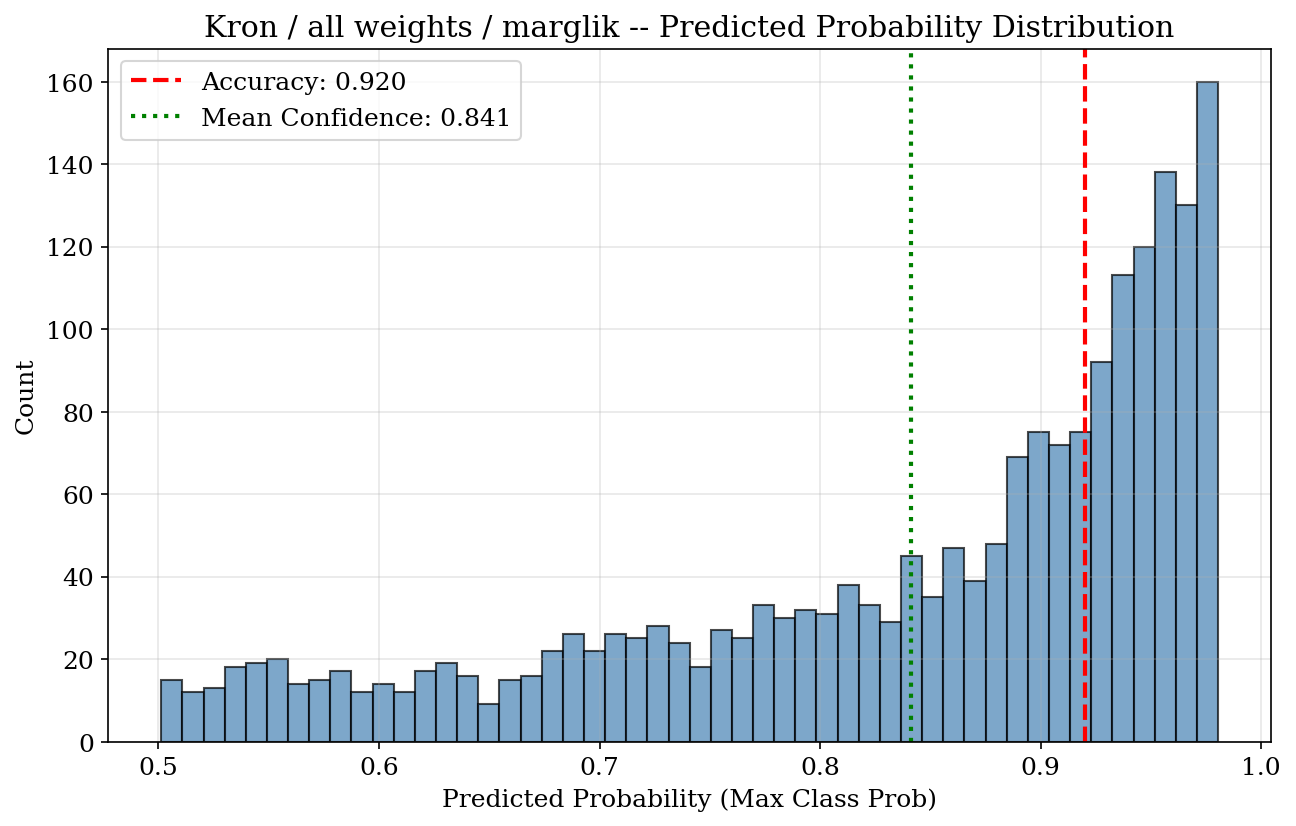
\includegraphics[width=\linewidth]{marglik_kron_all_weights_histogram.png}
\centerline{\tiny Prediction confidence histogram}
\end{columns}
\end{frame}

% ------------------------------------------------------------
\begin{frame}{Full / LL / ML}
\begin{columns}
\column{0.5\textwidth}
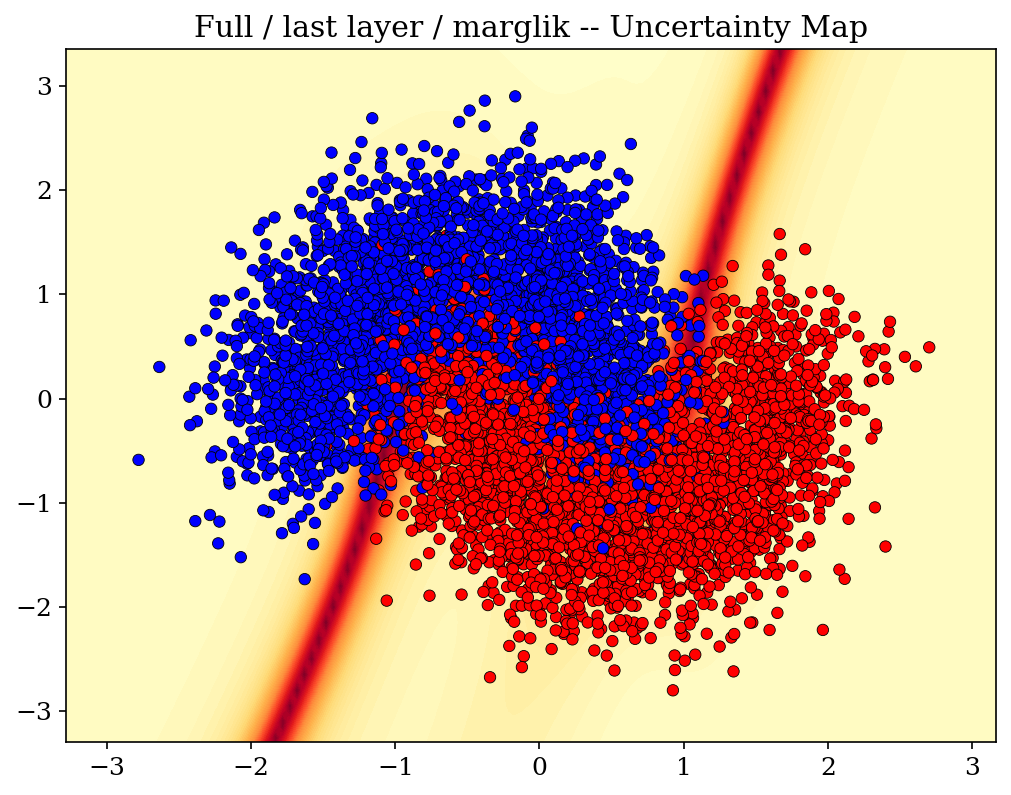
\includegraphics[width=\linewidth]{marglik_full_last_layer_uncertainty.png}
\centerline{\tiny Uncertainty map ($1 - \max_c \hat{p}_c$)}
\column{0.5\textwidth}
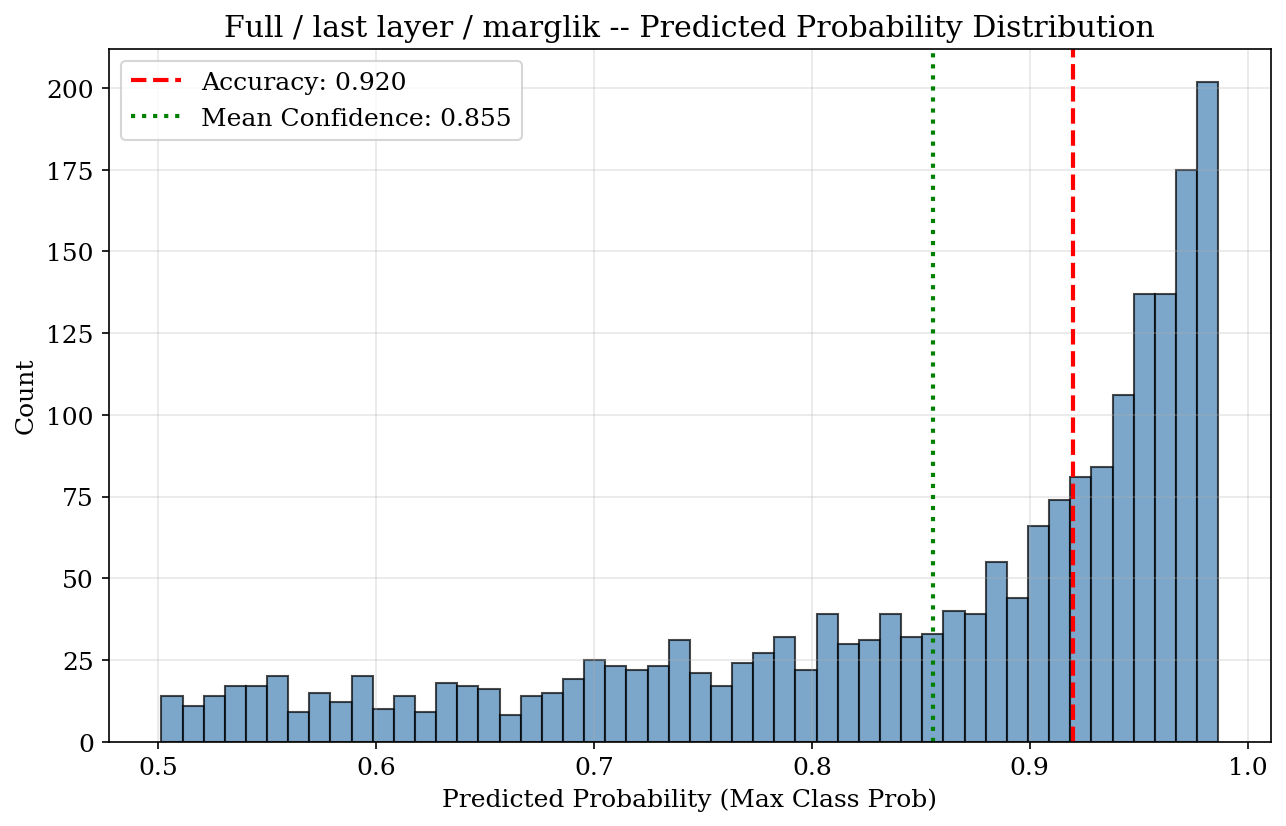
\includegraphics[width=\linewidth]{marglik_full_last_layer_histogram.png}
\centerline{\tiny Prediction confidence histogram}
\end{columns}
\end{frame}

% ------------------------------------------------------------
\begin{frame}{Kron / LL / ML}
\begin{columns}
\column{0.5\textwidth}
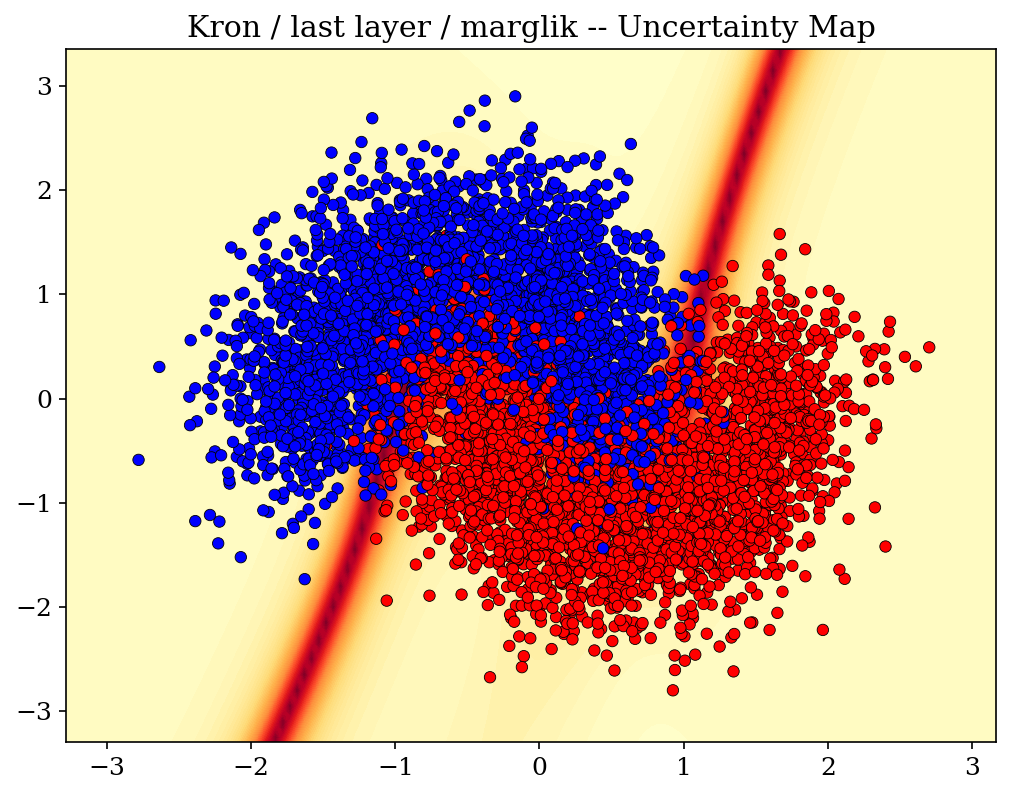
\includegraphics[width=\linewidth]{marglik_kron_last_layer_uncertainty.png}
\centerline{\tiny Uncertainty map ($1 - \max_c \hat{p}_c$)}
\column{0.5\textwidth}
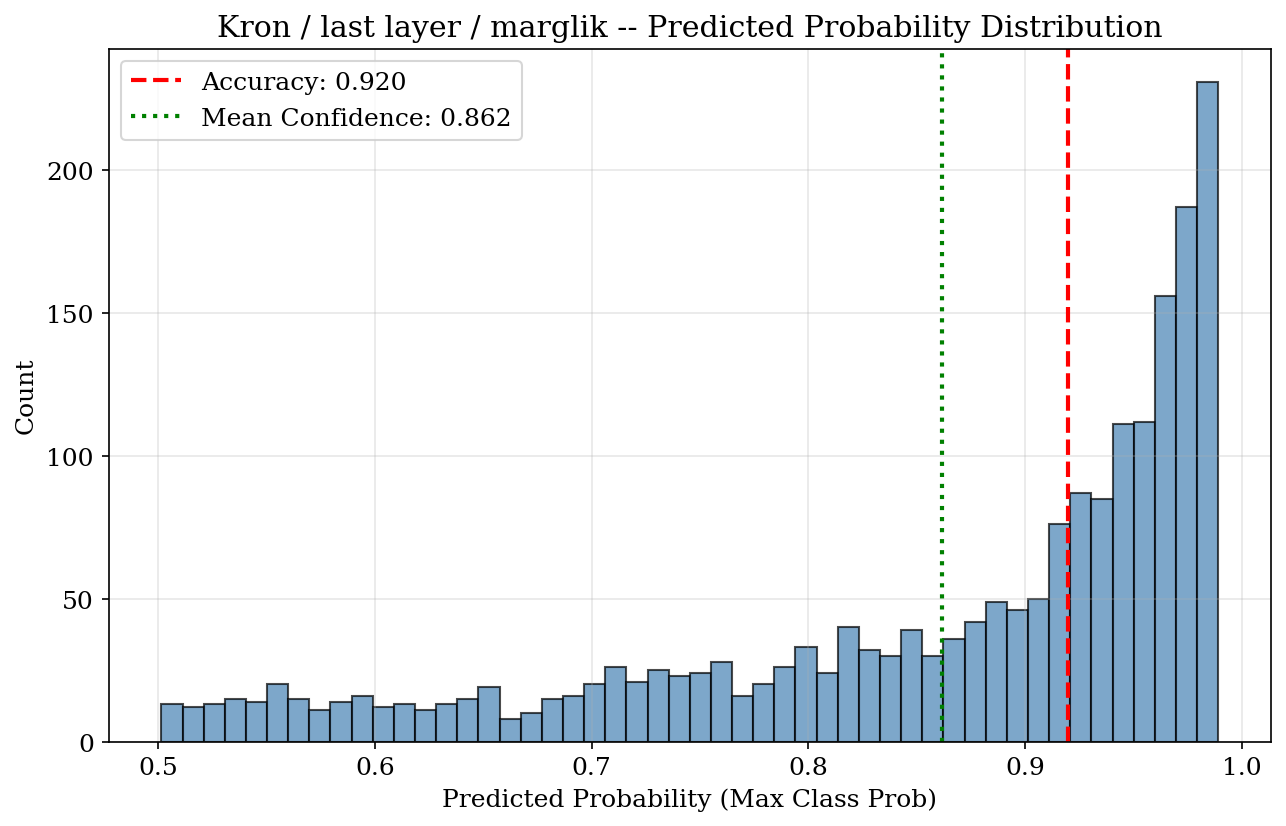
\includegraphics[width=\linewidth]{marglik_kron_last_layer_histogram.png}
\centerline{\tiny Prediction confidence histogram}
\end{columns}
\end{frame}

% ------------------------------------------------------------
\begin{frame}{Bayesian Variational Inference: Configurations}
\begin{table}
\centering
\small
\begin{tabular}{lll}
\toprule
\textbf{Model} & \textbf{Init} & \textbf{Loss} \\
\midrule
Flipout & scratch & ELBO \\
Flipout & scratch & ELBO+AvUC \\
Flipout & MOPED & ELBO \\
Flipout & MOPED & ELBO+AvUC \\
BBB & scratch & ELBO \\
BBB & scratch & ELBO+AvUC \\
BBB & MOPED & ELBO \\
BBB & MOPED & ELBO+AvUC \\
\bottomrule
\end{tabular}
\end{table}
\vspace{0.2cm}
All use 5 posterior samples at inference, 2 hidden layers (50 units), ReLU.
\end{frame}

% ------------------------------------------------------------
\begin{frame}{Bayesian Calibration Metrics}
\begin{threeparttable}
\centering
\small
\begin{tabular}{lcccc}
\toprule
\textbf{Variant} & \textbf{BS$\downarrow$} & \textbf{ECE$\downarrow$} & \textbf{U-MAE$\downarrow$} & \textbf{U-Corr$\uparrow$} \\
\midrule
Flipout / scr / ELBO & 0.0579 & 0.0179 & 0.018 & 0.988 \\
Flipout / scr / AvUC & 0.0589 & 0.0139 & 0.014 & 0.953 \\
Flipout / MOP / ELBO & 0.0591 & 0.0188 & 0.019 & 0.935 \\
Flipout / MOP / AvUC & 0.0587 & 0.0100 & 0.010 & 0.990 \\
BBB / scr / ELBO & 0.0579 & 0.0187 & 0.019 & 0.983 \\
BBB / scr / AvUC & 0.0952 & 0.0277 & 0.028 & 0.965 \\
BBB / MOP / ELBO & 0.0580 & 0.0145 & 0.015 & 0.967 \\
BBB / MOP / AvUC & 0.0567 & 0.0142 & 0.014 & 0.941 \\
\bottomrule
\end{tabular}
\end{threeparttable}
\end{frame}

% ------------------------------------------------------------
\begin{frame}{Bayesian Computational Metrics}
\begin{threeparttable}
\centering
\small
\begin{tabular}{lcccc}
\toprule
\textbf{Variant} & \textbf{MaxGap$\downarrow$} & \textbf{U-MSE$\downarrow$} & \textbf{Fit (s)} & \textbf{Inf (s)} \\
\midrule
Flipout / scr / ELBO & 0.069 & 0.00046 & 19.1 & 0.064 \\
Flipout / scr / AvUC & 0.134 & 0.00084 & 80.4 & 0.065 \\
Flipout / MOP / ELBO & 0.113 & 0.00088 & 20.0 & 0.063 \\
Flipout / MOP / AvUC & 0.078 & 0.00029 & 90.1 & 0.064 \\
BBB / scr / ELBO & 0.051 & 0.00058 & 23.2 & 0.051 \\
BBB / scr / AvUC & 0.102 & 0.00092 & 73.3 & 0.050 \\
BBB / MOP / ELBO & 0.130 & 0.00056 & 15.9 & 0.055 \\
BBB / MOP / AvUC & 0.123 & 0.00090 & 68.7 & 0.050 \\
\bottomrule
\end{tabular}
{\small
\begin{tablenotes}
\item[scr] scratch (random init); \;[MOP] MOPED init ($\delta=0.5$);
\item[AvUC] ELBO + AvUC loss ($\lambda=0.1$); \;[Fit/Inf] training and inference time.
\end{tablenotes}}
\end{threeparttable}
\end{frame}

% ------------------------------------------------------------
\begin{frame}{Flipout / scratch / ELBO}
\begin{columns}
\column{0.5\textwidth}
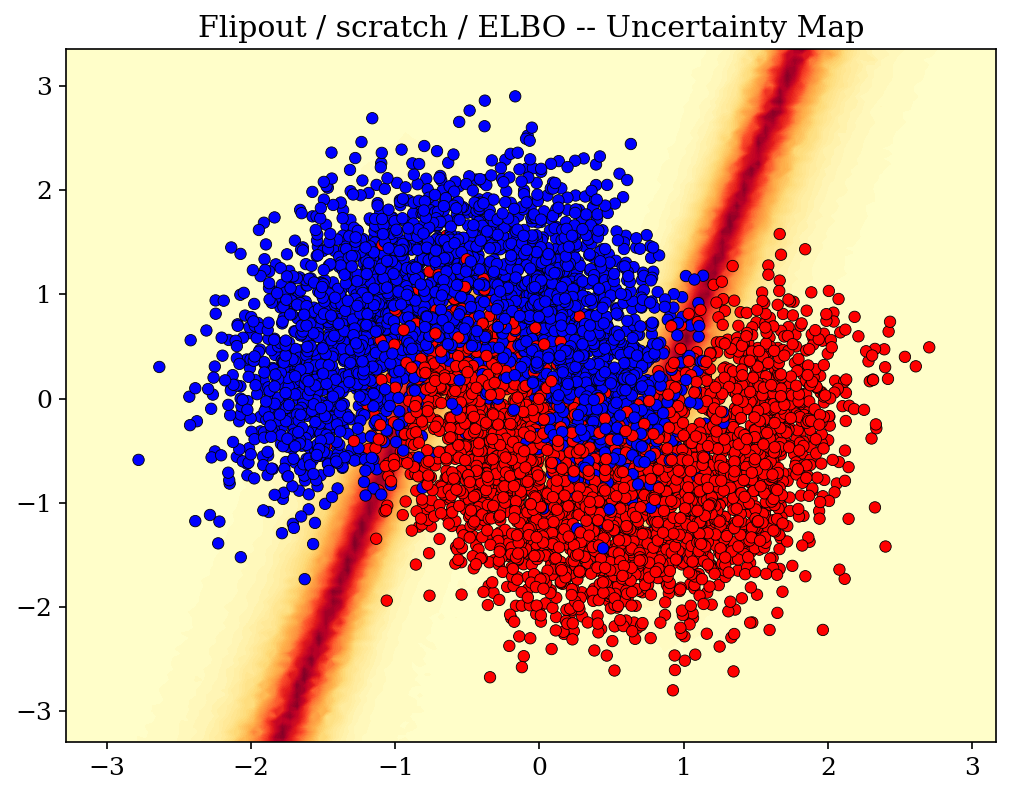
\includegraphics[width=\linewidth]{flipout_scratch_elbo_uncertainty.png}
\centerline{\tiny Uncertainty map ($1 - \max_c \hat{p}_c$)}
\column{0.5\textwidth}
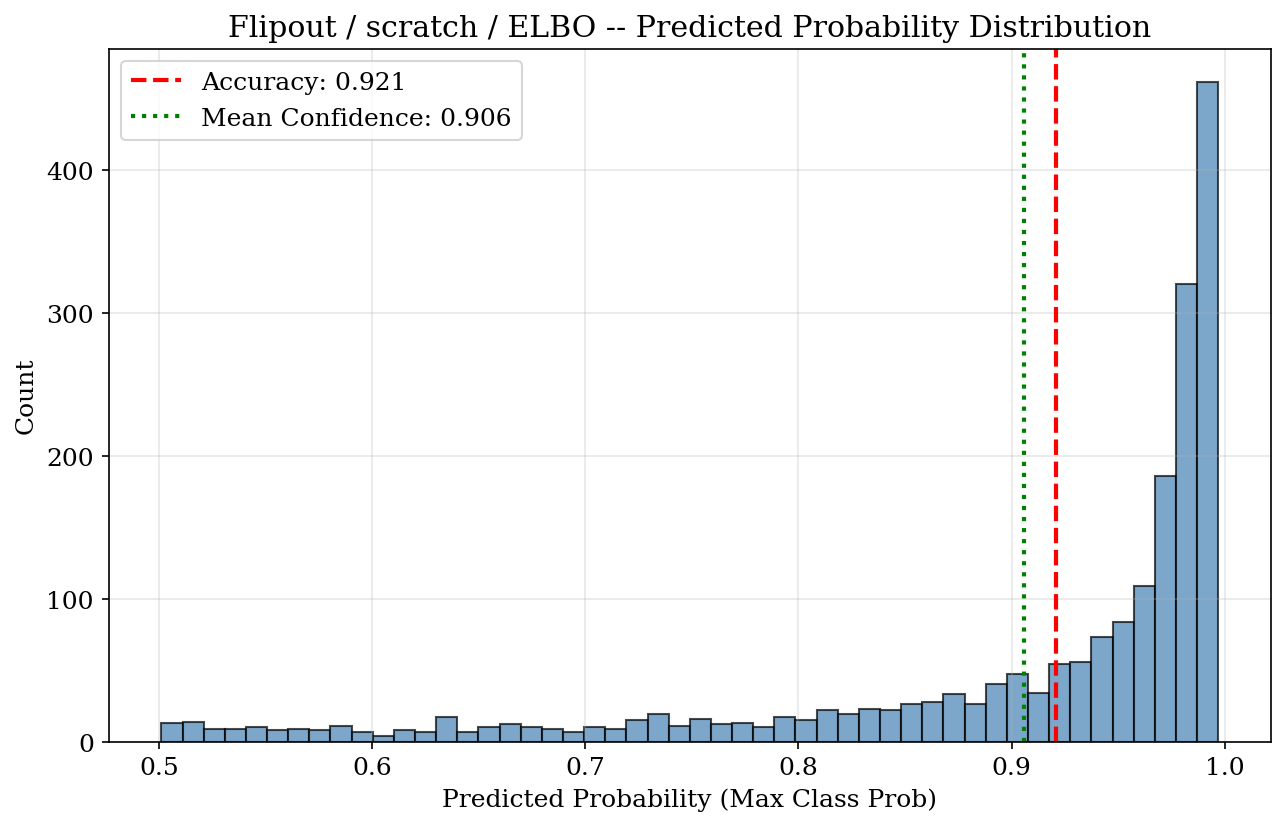
\includegraphics[width=\linewidth]{flipout_scratch_elbo_histogram.png}
\centerline{\tiny Prediction confidence histogram}
\end{columns}
\end{frame}

% ------------------------------------------------------------
\begin{frame}{Flipout / scratch / AvUC}
\begin{columns}
\column{0.5\textwidth}
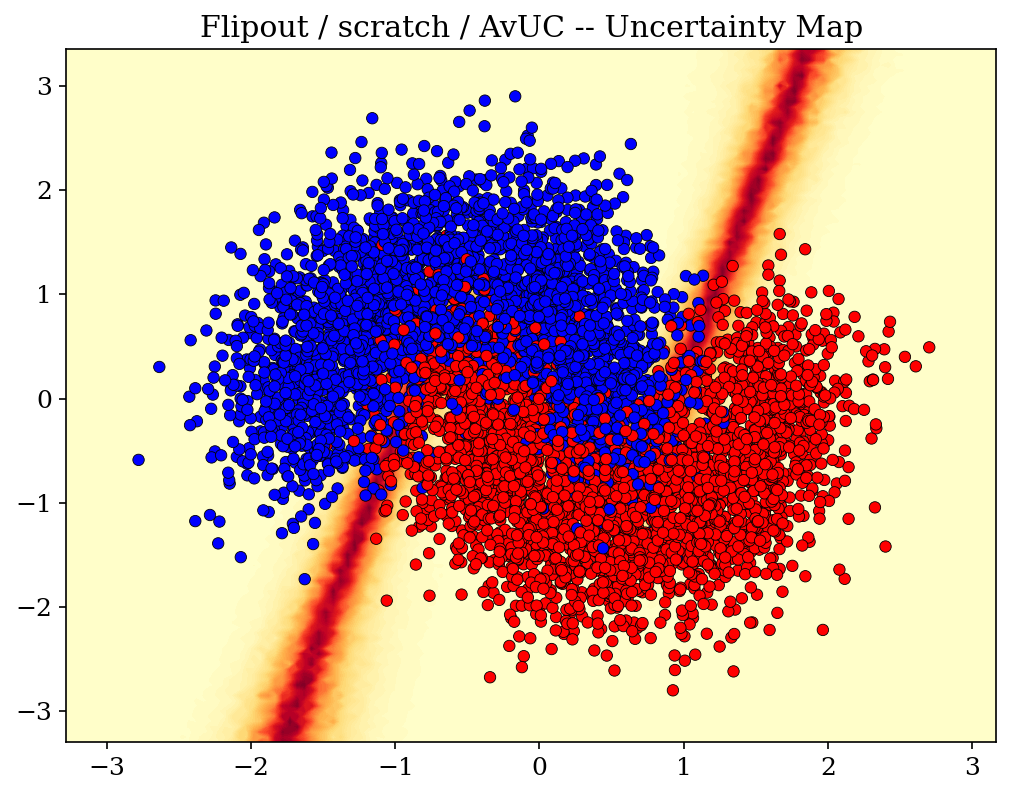
\includegraphics[width=\linewidth]{flipout_scratch_avuc_uncertainty.png}
\centerline{\tiny Uncertainty map ($1 - \max_c \hat{p}_c$)}
\column{0.5\textwidth}
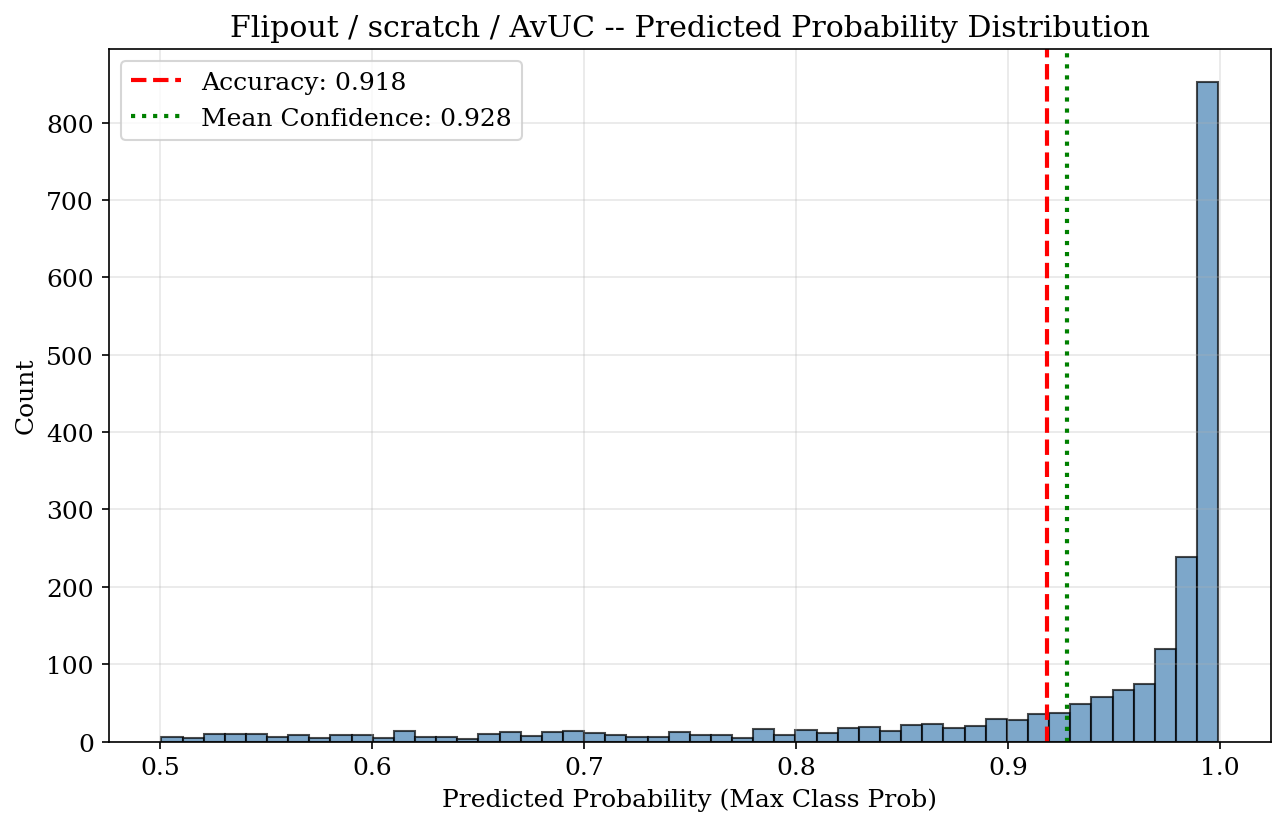
\includegraphics[width=\linewidth]{flipout_scratch_avuc_histogram.png}
\centerline{\tiny Prediction confidence histogram}
\end{columns}
\end{frame}

% ------------------------------------------------------------
\begin{frame}{Flipout / MOP / ELBO}
\begin{columns}
\column{0.5\textwidth}
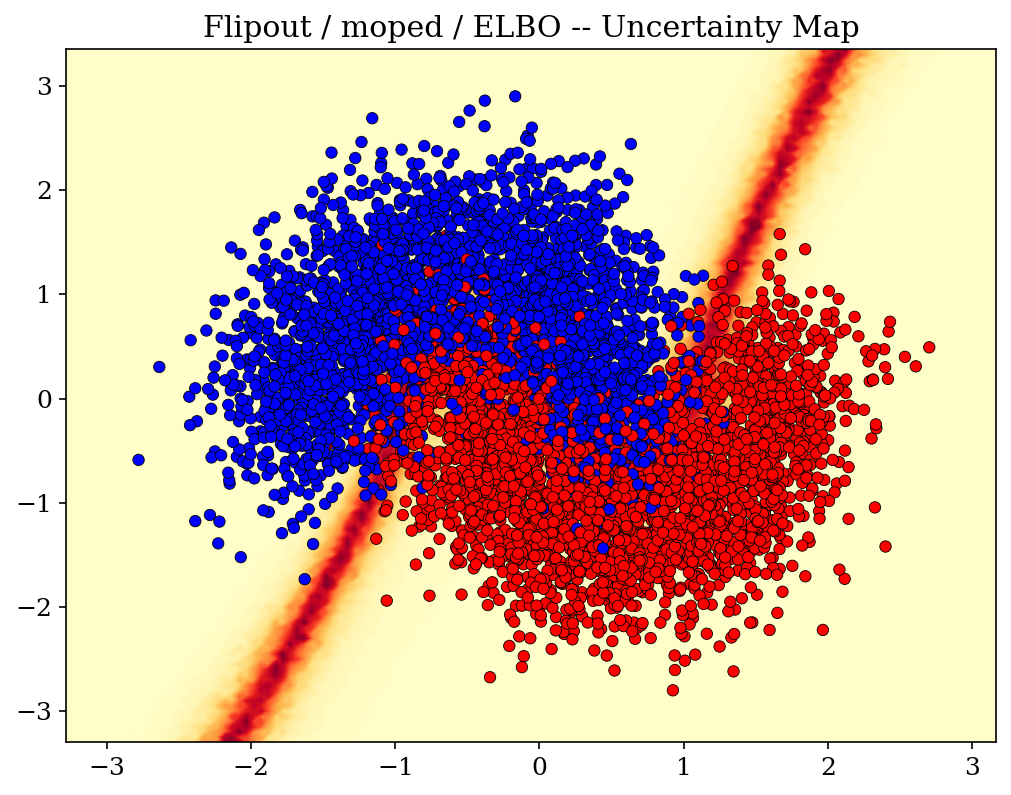
\includegraphics[width=\linewidth]{flipout_moped_elbo_uncertainty.png}
\centerline{\tiny Uncertainty map ($1 - \max_c \hat{p}_c$)}
\column{0.5\textwidth}
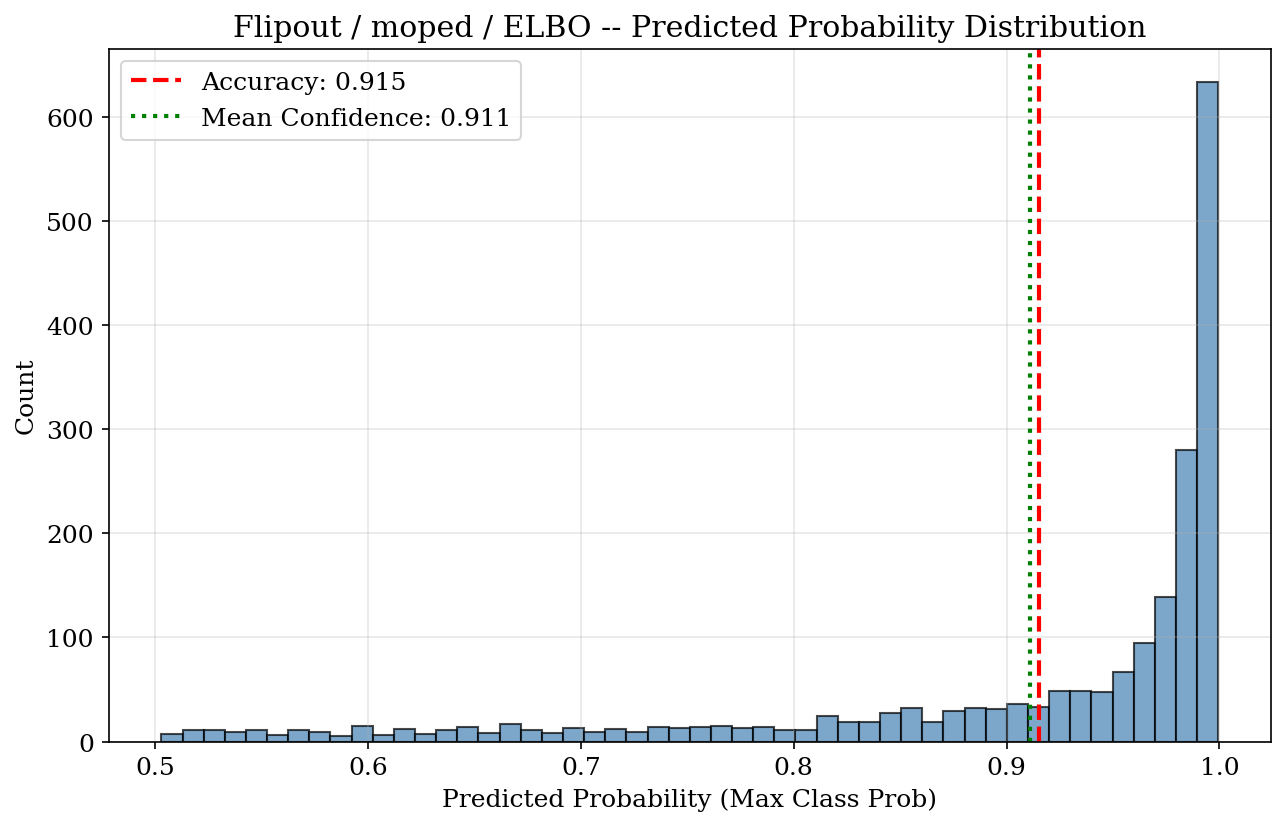
\includegraphics[width=\linewidth]{flipout_moped_elbo_histogram.png}
\centerline{\tiny Prediction confidence histogram}
\end{columns}
\end{frame}

% ------------------------------------------------------------
\begin{frame}{Flipout / MOP / AvUC}
\begin{columns}
\column{0.5\textwidth}
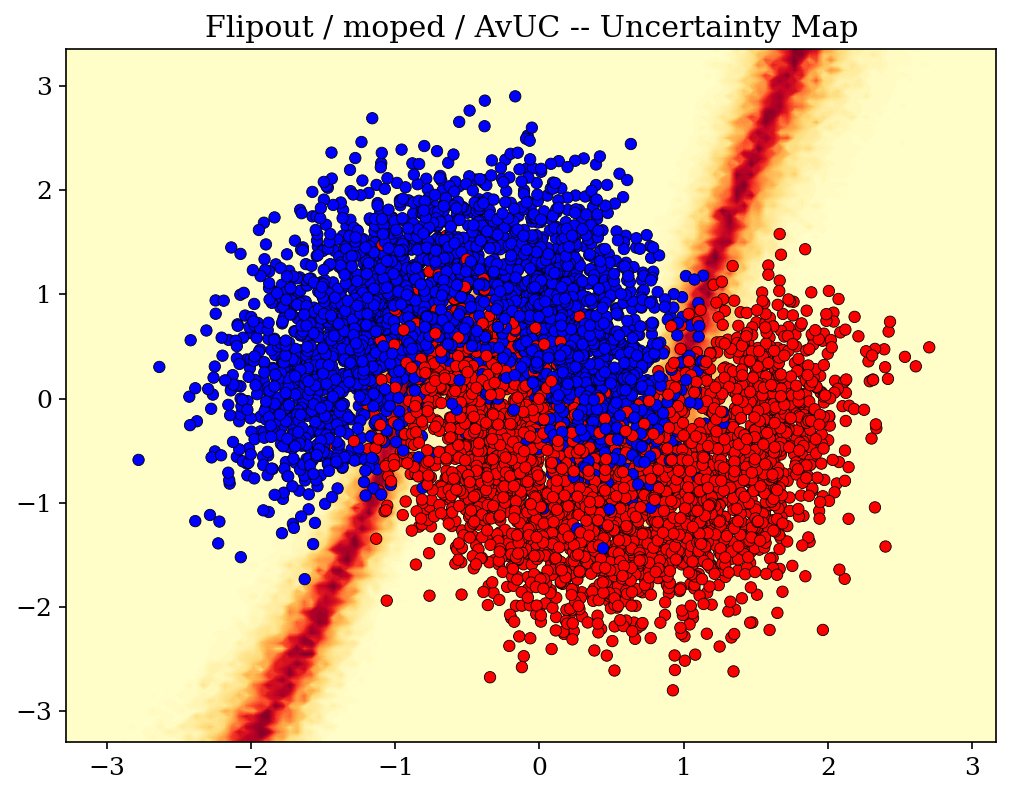
\includegraphics[width=\linewidth]{flipout_moped_avuc_uncertainty.png}
\centerline{\tiny Uncertainty map ($1 - \max_c \hat{p}_c$)}
\column{0.5\textwidth}
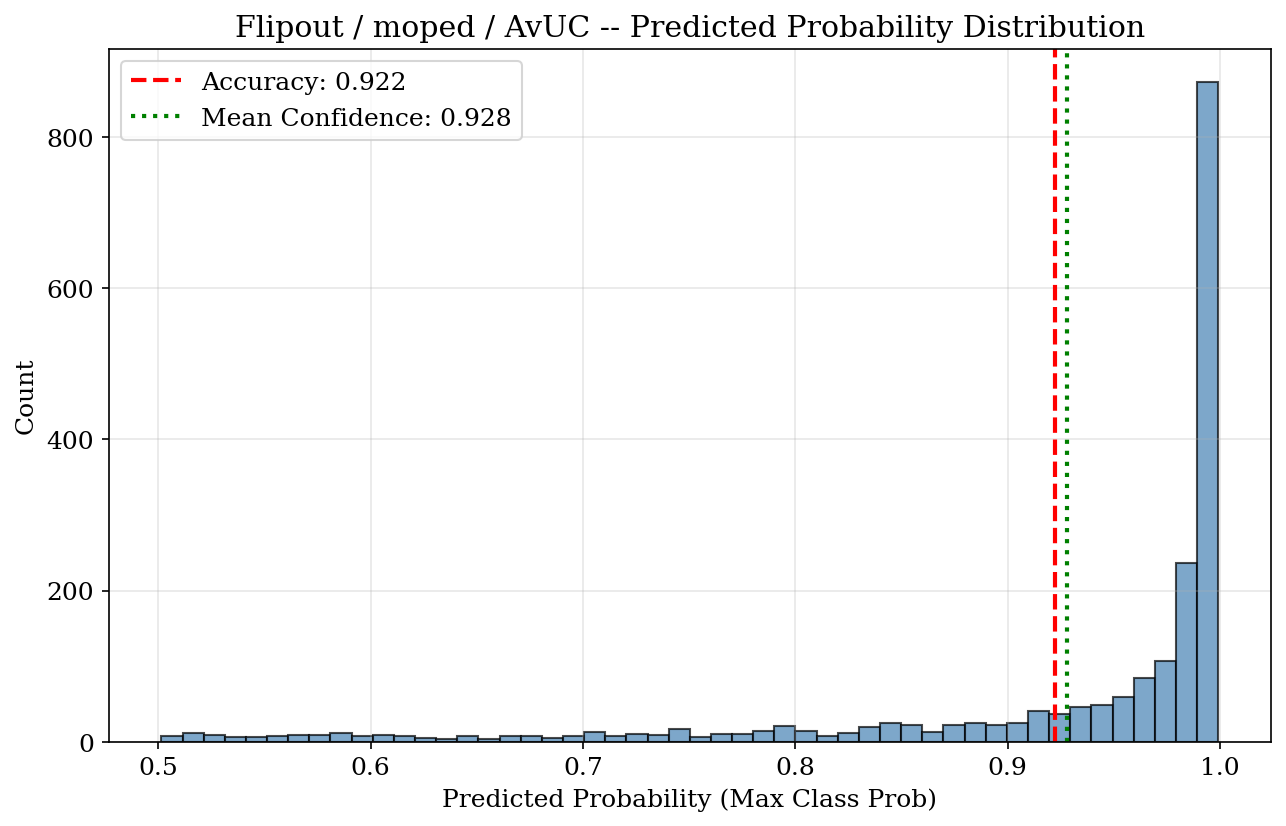
\includegraphics[width=\linewidth]{flipout_moped_avuc_histogram.png}
\centerline{\tiny Prediction confidence histogram}
\end{columns}
\end{frame}

% ------------------------------------------------------------
\begin{frame}{BBB / scratch / ELBO}
\begin{columns}
\column{0.5\textwidth}
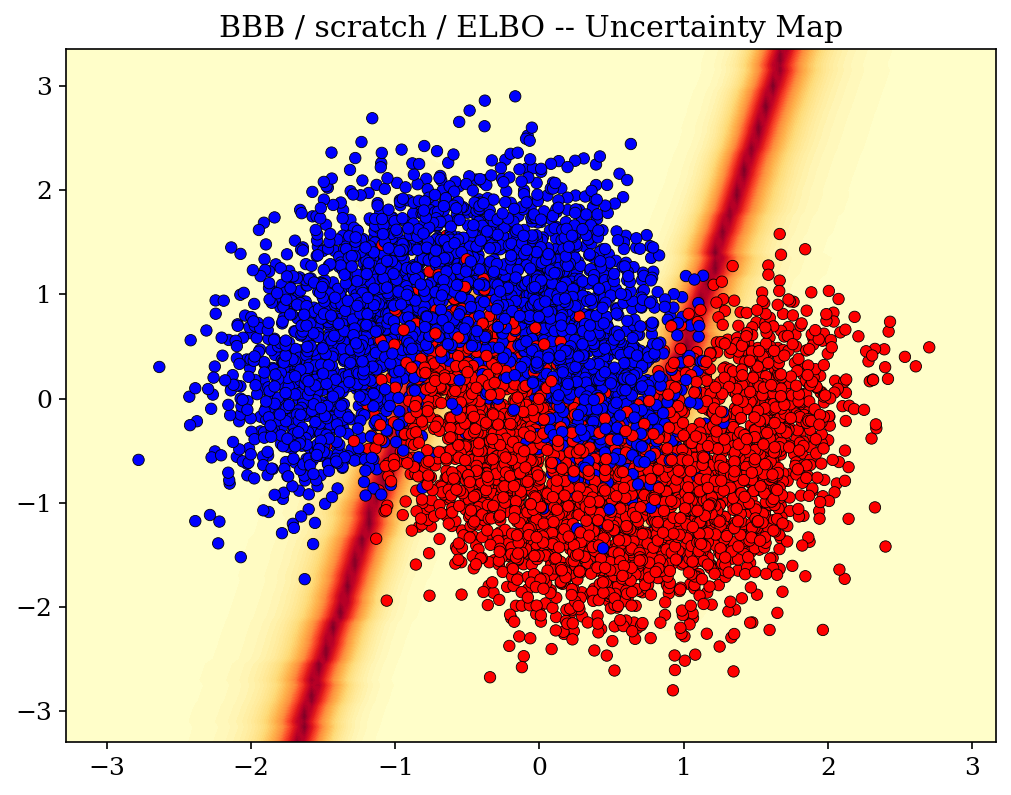
\includegraphics[width=\linewidth]{bbb_scratch_elbo_uncertainty.png}
\centerline{\tiny Uncertainty map ($1 - \max_c \hat{p}_c$)}
\column{0.5\textwidth}
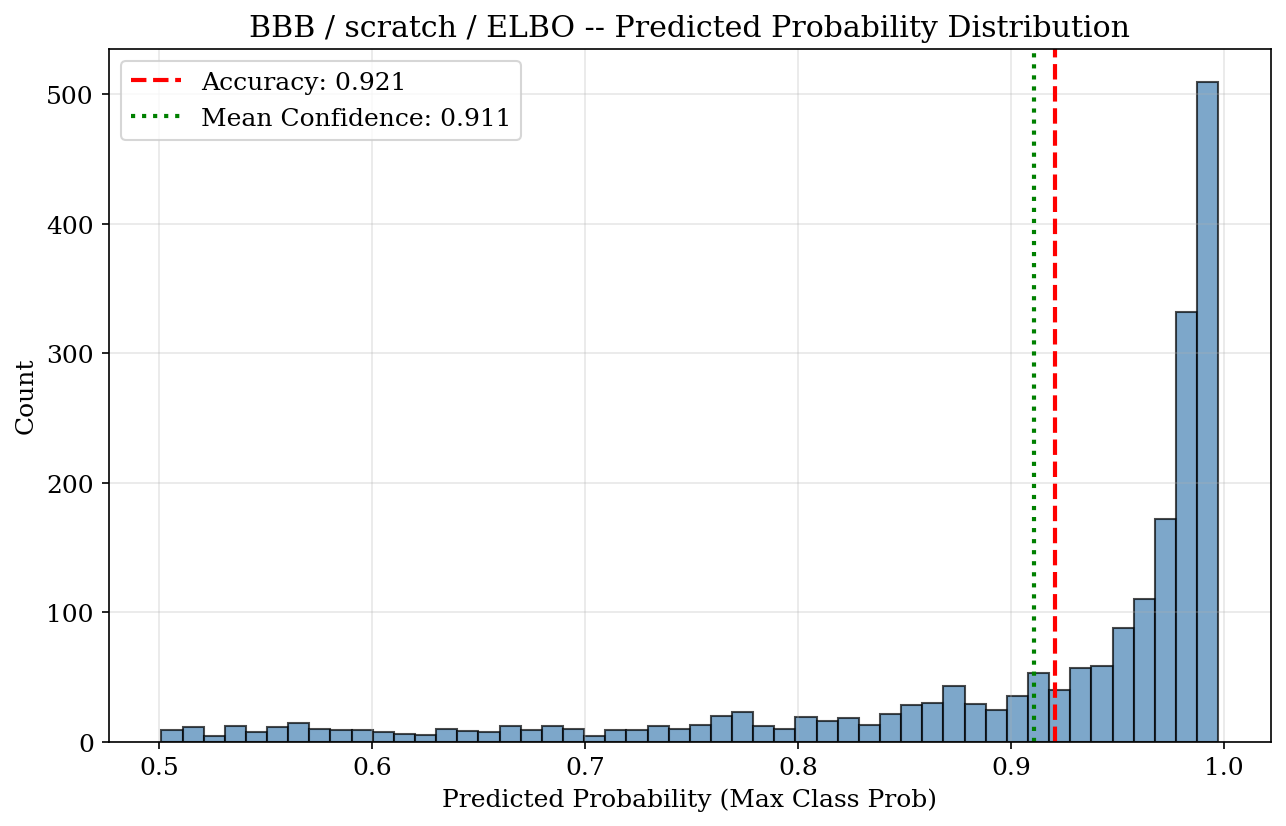
\includegraphics[width=\linewidth]{bbb_scratch_elbo_histogram.png}
\centerline{\tiny Prediction confidence histogram}
\end{columns}
\end{frame}

% ------------------------------------------------------------
\begin{frame}{BBB / scratch / AvUC}
\begin{columns}
\column{0.5\textwidth}
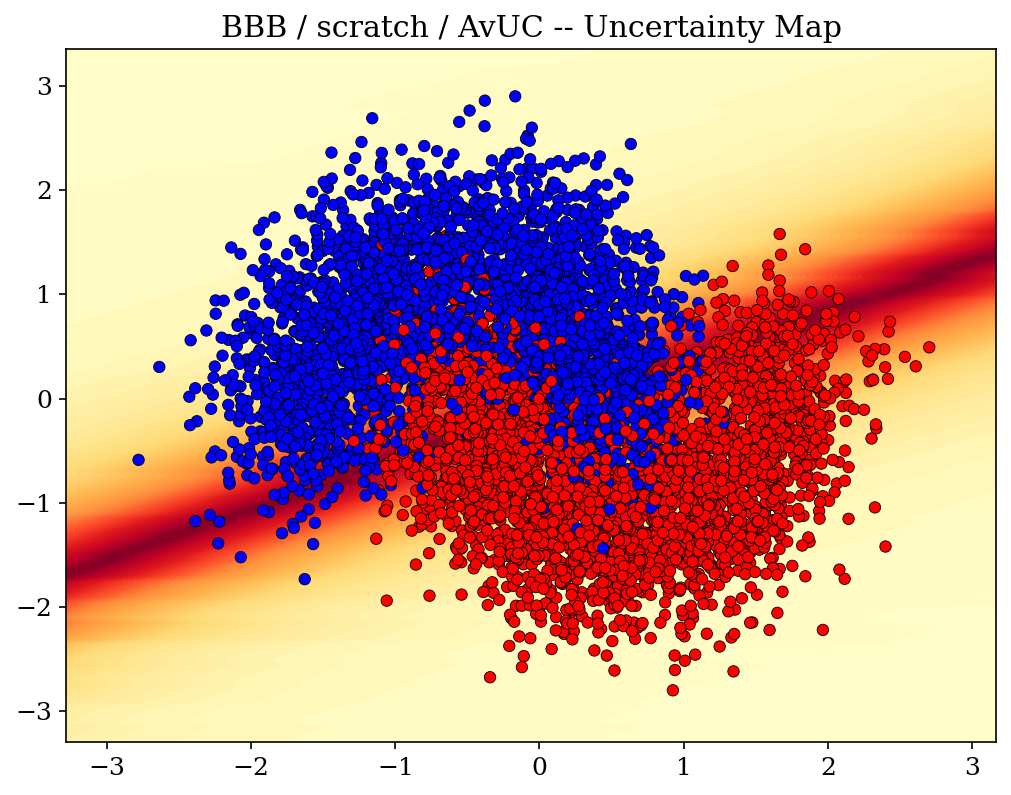
\includegraphics[width=\linewidth]{bbb_scratch_avuc_uncertainty.png}
\centerline{\tiny Uncertainty map ($1 - \max_c \hat{p}_c$)}
\column{0.5\textwidth}
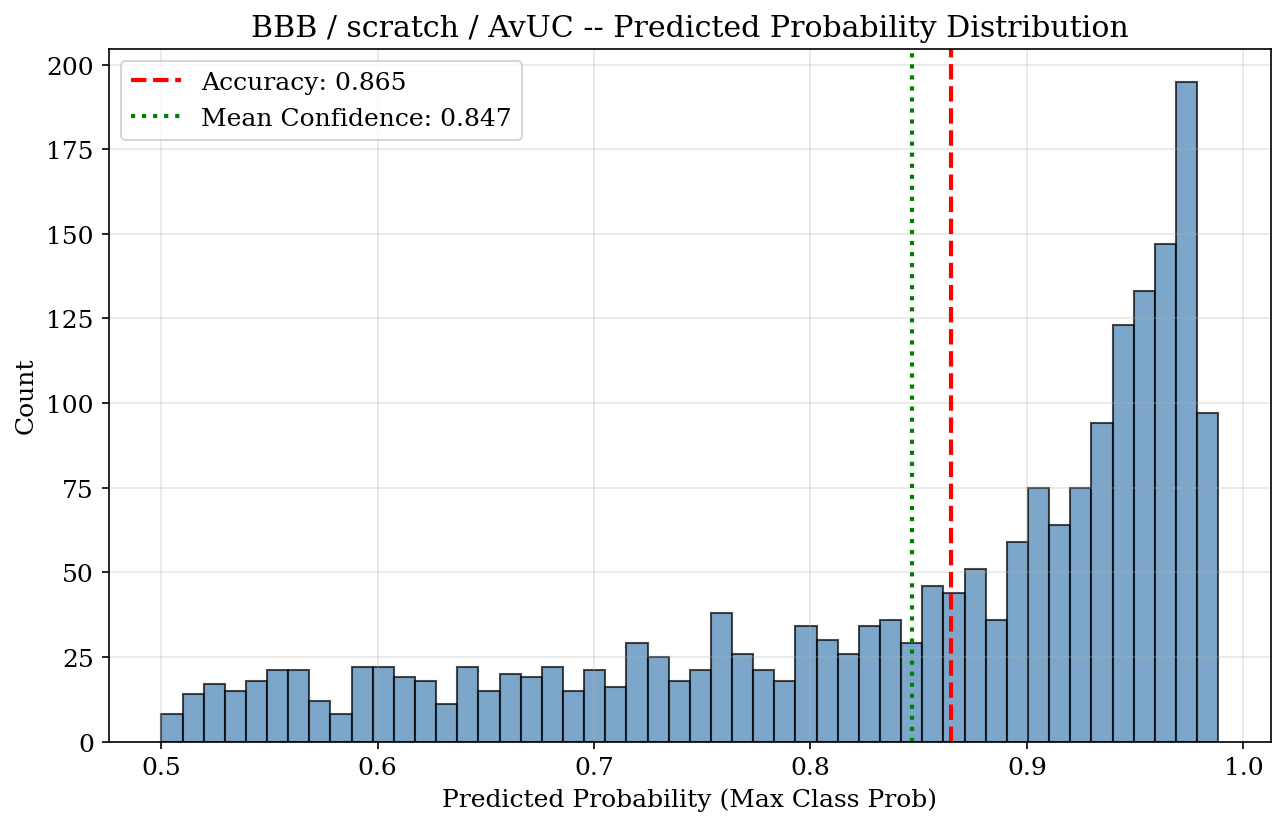
\includegraphics[width=\linewidth]{bbb_scratch_avuc_histogram.png}
\centerline{\tiny Prediction confidence histogram}
\end{columns}
\end{frame}

% ------------------------------------------------------------
\begin{frame}{BBB / MOP / ELBO}
\begin{columns}
\column{0.5\textwidth}
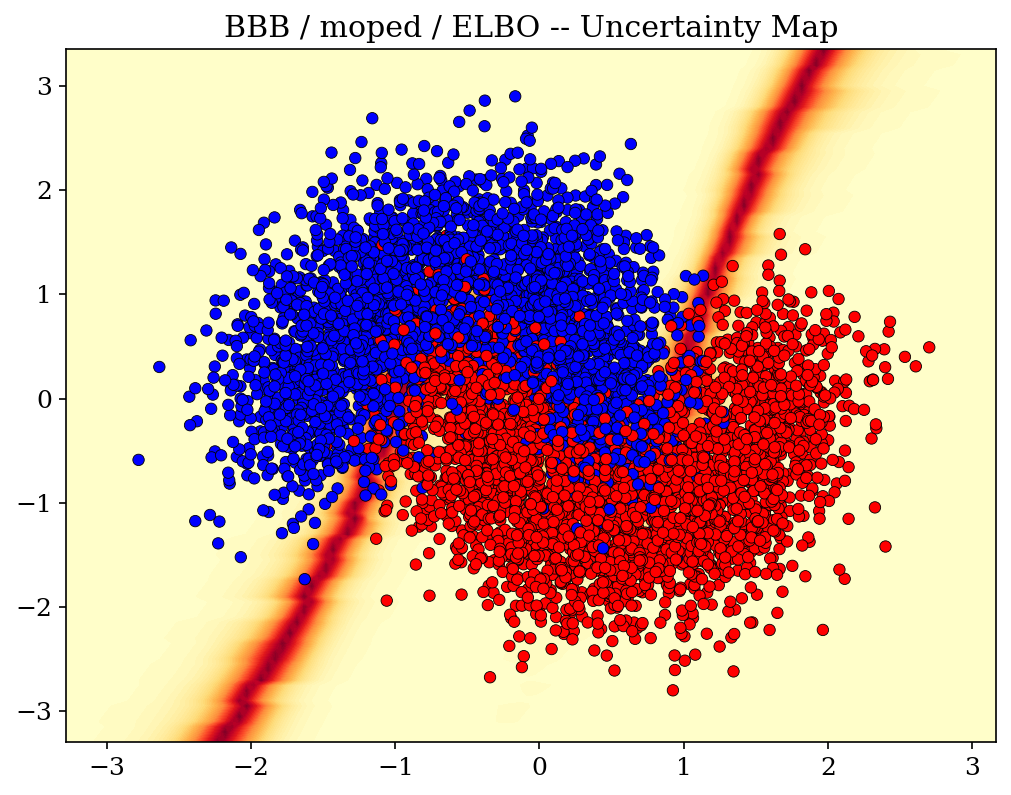
\includegraphics[width=\linewidth]{bbb_moped_elbo_uncertainty.png}
\centerline{\tiny Uncertainty map ($1 - \max_c \hat{p}_c$)}
\column{0.5\textwidth}
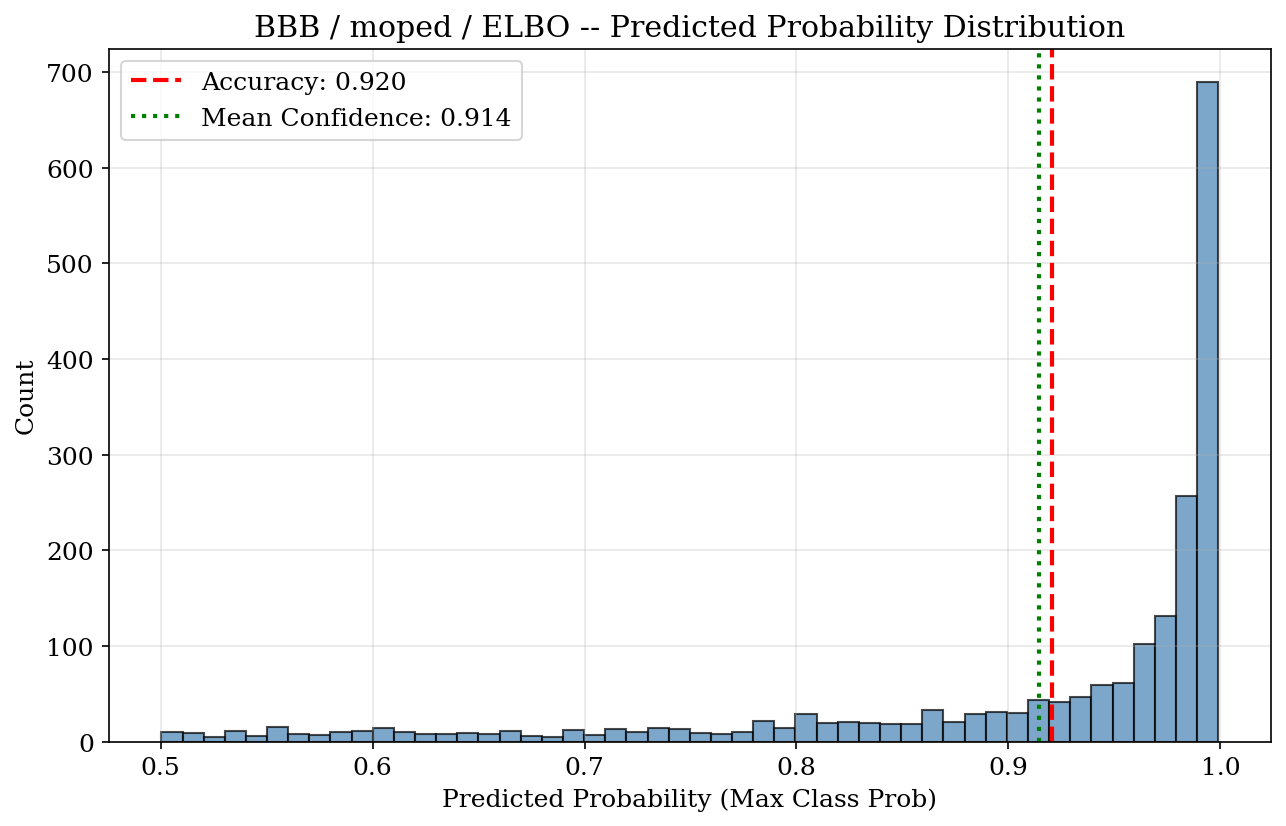
\includegraphics[width=\linewidth]{bbb_moped_elbo_histogram.png}
\centerline{\tiny Prediction confidence histogram}
\end{columns}
\end{frame}

% ------------------------------------------------------------
\begin{frame}{BBB / MOP / AvUC}
\begin{columns}
\column{0.5\textwidth}
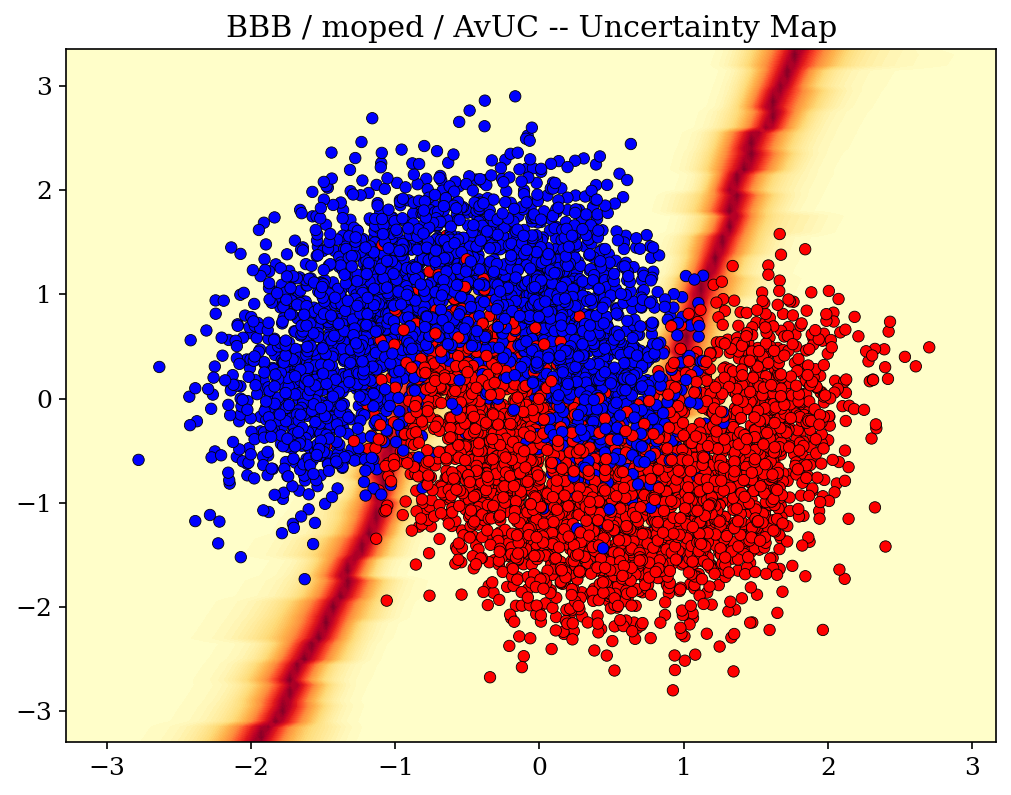
\includegraphics[width=\linewidth]{bbb_moped_avuc_uncertainty.png}
\centerline{\tiny Uncertainty map ($1 - \max_c \hat{p}_c$)}
\column{0.5\textwidth}
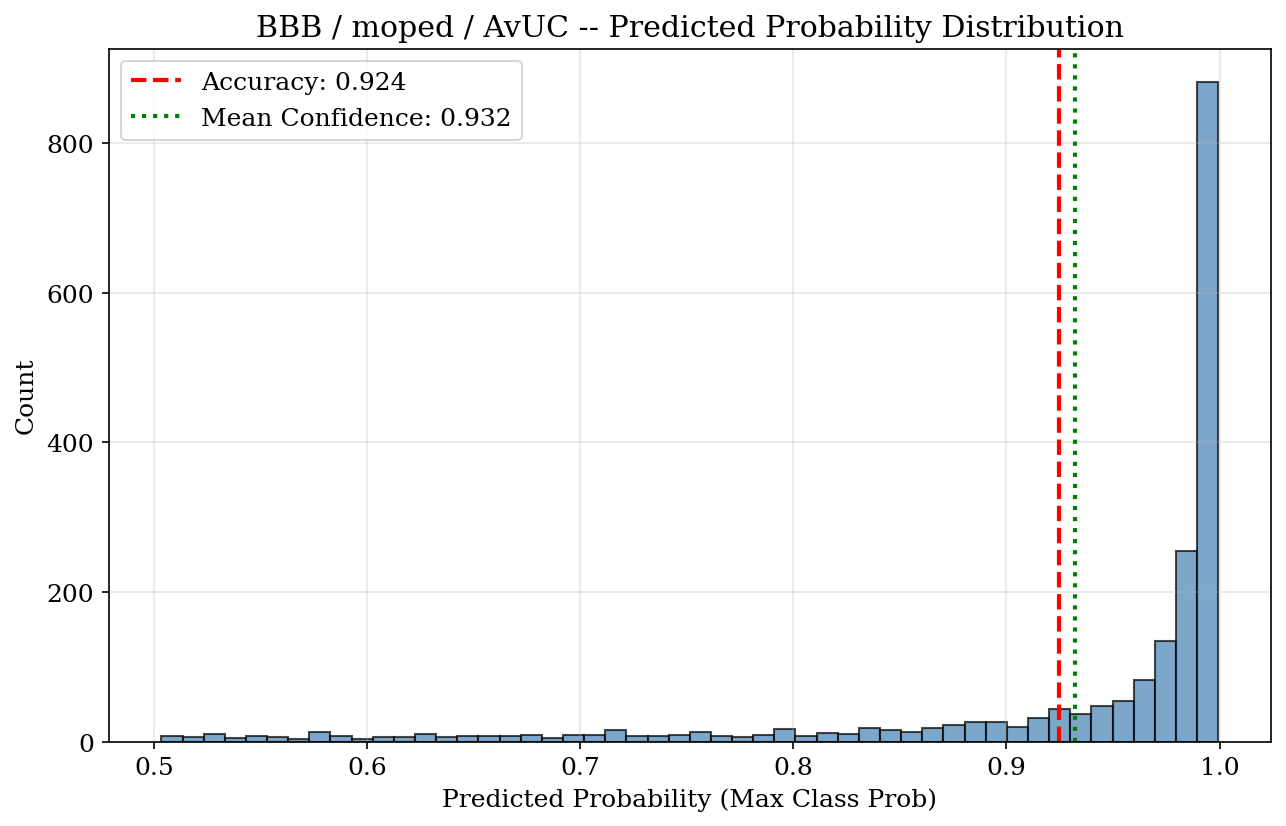
\includegraphics[width=\linewidth]{bbb_moped_avuc_histogram.png}
\centerline{\tiny Prediction confidence histogram}
\end{columns}
\end{frame}

% ------------------------------------------------------------
\begin{frame}{Cross-Comparison: Laplace vs Variational}
\begin{threeparttable}
\centering
\small
\begin{tabular}{lccccc}
\toprule
\textbf{Method} & \textbf{BS$\downarrow$} & \textbf{ECE$\downarrow$} & \textbf{U-Corr$\uparrow$} & \textbf{Fit (s)} & \textbf{Inf (s)} \\
\midrule
\textit{Laplace} \\
\hspace{0.2em}Kron / LL / GS & 0.0564 & 0.0101 & 0.959 & 0.43 & 0.001 \\
\hspace{0.2em}Kron / LL / ML & 0.0613 & 0.0637 & 0.938 & 0.44 & 0.001 \\
\textit{Flipout MOPED} \\
\hspace{0.2em}ELBO & 0.0591 & 0.0188 & 0.935 & 20.0 & 0.063 \\
\hspace{0.2em}AvUC & 0.0587 & 0.0100 & 0.990 & 90.1 & 0.064 \\
\textit{BBB MOPED} \\
\hspace{0.2em}ELBO & 0.0580 & 0.0145 & 0.967 & 15.9 & 0.055 \\
\hspace{0.2em}AvUC & 0.0567 & 0.0142 & 0.941 & 68.7 & 0.050 \\
\bottomrule
\end{tabular}
{\small
\begin{tablenotes}
\item Kron LL GS achieves ECE matching Flipout AvUC (0.010) at 200$\times$ faster fit time.
\item Marglik underperforms gridsearch here; SVI AvUC improves ECE over ELBO in most cases.
\end{tablenotes}}
\end{threeparttable}
\end{frame}

% ------------------------------------------------------------
\begin{frame}{OOD / ID Uncertainty Analysis}
\begin{threeparttable}
\centering
\small
\begin{tabular}{lcccc}
\toprule
\textbf{Variant} & \textbf{ID $1{-}c$} & \textbf{OOD $1{-}c$} & \textbf{ID Epist} & \textbf{$\Delta$Epist} \\
\midrule
Diag / all / GS & 0.079 & 0.0004 & 0.0002 & $-2\!\times\!10^{-4}$ \\
Full / all / GS & 0.079 & 0.0004 & 0.0001 & $-1\!\times\!10^{-4}$ \\
Kron / all / GS & 0.079 & 0.0004 & 0.0002 & $-2\!\times\!10^{-4}$ \\
Full / LL / GS & 0.079 & 0.0004 & $6\!\times\!10^{-5}$ & $-6\!\times\!10^{-5}$ \\
Kron / LL / GS & 0.079 & 0.0004 & $7\!\times\!10^{-5}$ & $-7\!\times\!10^{-5}$ \\
Flipout MOP AvUC & 0.073 & 0.0041 & 0.0355 & $-0.032$ \\
BBB MOP AvUC & 0.067 & 0.0071 & 0.0347 & $-0.026$ \\
\bottomrule
\end{tabular}
{\small
\begin{tablenotes}
\item[$1{-}c$] Mean uncertainty ($1 - \max_c \hat{p}_c$); \;[Epist] Epistemic uncertainty (predictive variance)
\item[$\Delta$Epist] OOD epistemic minus ID epistemic. Negative $\Delta$Epist indicates posterior collapse outside the training region.
\end{tablenotes}}
\end{threeparttable}
\end{frame}

\end{document}
